\documentclass[11pt,compress,professionalfonts]{beamer}
\usetheme{metropolis}

\usepackage[]{graphicx}
\usepackage[]{color}

\usepackage{ctable}
\usepackage{hyperref}
\usepackage{dcolumn}
\usepackage{booktabs}

\usepackage{mathspec}
\setsansfont{Avenir Next}[BoldFont={* Demi Bold}]
\setmonofont[Scale = MatchLowercase,Mapping=tex-ansi]{Inconsolata}
\setmathfont(Digits,Latin,Greek){Avenir Next}
\newfontface\fancy{Avenir Light}[Mapping=tex-ansi]

\definecolor{darkgray}{rgb}{0.5,0.5,0.5}
\definecolor{darkblue}{rgb}{0.000,0.251,0.502}
\definecolor{bloodred}{rgb}{0.502,0.000,0.000}
\definecolor{darkgreen}{rgb}{0.000,0.502,0.0}
\definecolor{verylightgray}{rgb}{0.95,0.95,0.95}

\setbeamerfont{frametitle}{size=\Large,family=\fancy}
\setbeamercolor{frametitle}{fg=bloodred, bg=verylightgray}
\setbeamerfont{title}{family=\fancy,size=\Large}
\setbeamercolor{title}{fg=bloodred}
\setbeamercolor{background canvas}{bg=white}
\setbeamercolor{normal text}{fg=black}
\setbeamercolor{title separator}{fg=darkgray}

\metroset{progressbar=none,numbering=none}

\IfFileExists{upquote.sty}{\usepackage{upquote}}{}

%% bullet free bullet points
\newcommand{\ita}{\begin{itemize}}
\newcommand{\itm}{\item[]}
\newcommand{\itz}{\end{itemize}}

% graphics file in the pics subdirectory please
\graphicspath{{./pics/}}

\title{Computer-assisted content analysis}
\author{Will Lowe ~~Princeton University\\James Lo ~~ University of Southern California}
\date{Part 1}
\begin{document}

\maketitle


\begin{frame}[t]\frametitle{Practicalities: Materials}

We have a website:
\ita
\itm \url{http://conjugateprior.org/teaching/texas/}
\itm Password: quantext
\itz

\end{frame}
\begin{frame}[t]\frametitle{Practicalities: Labs}

\centerline{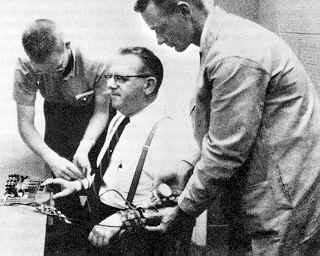
\includegraphics[scale=0.25]{pictures/milgram-subject}}

Worked examples (usually in the tools themselves and also in an R wrapper)

\end{frame}
\begin{frame}[t]\frametitle{Menu}

Session 0: How could this possibly work?

Session 1: Dictionary-based `classical' content analysis and topic models

Session 2: Classification and evaluation

Session 3: Scaling Models


\end{frame}
\begin{frame}[t]\frametitle{Focus}

Assumptions

Mechanics

Interpretation

Pitfalls


%\begin{frame}
%\frametitle{Menu}
%\small
%\tableofcontents
%\normalsize
%

\newpage

\end{frame}
\begin{frame}[t]\frametitle{Topics}
How to learn about
\ita
\itm party platforms
\itm legislative agendas
\itm parliamentary debates
\itm bloggers
\itm presidents
\itm international terrorists
\itz
by counting (lots of) words\ldots


\centerline{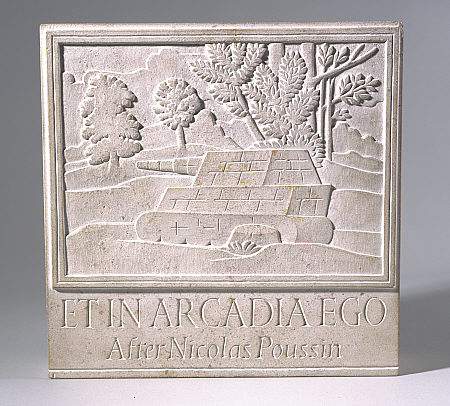
\includegraphics[scale=4]{pictures/etinarcadiaego}}

\end{frame}
\begin{frame}[t]\frametitle{The Transcendental Question}
~\\
What are the \textit{conditions for the possibility} of learning about these things by counting words?

\vfill
a.k.a how could this possibly work?

\end{frame}
\begin{frame}[t]\frametitle{Big Picture}

There is a \textsl{message} or \textit{content} that cannot be \textit{directly} observed, e.g.
\ita
\itm The topic of my lecture, my position on a political issue, the importance of defence issues to a some political party.
\itz
and \textit{behaviour}, including \textsl{linguistic behaviour}, e.g.
\ita
\itm yelling, muttering, cursing, lecturing
\itz
which \textit{can} be directly observed.

~\\
Focus on the \textit{expressed message} and the \textit{words}\ldots

\end{frame}
\begin{frame}[t]\frametitle{Communication}

To \textsl{communicate} a message $\theta$ -- to inform, persuade, demand, threaten, a producer (the speaker or writer) \textsl{generates} words of different kinds in different quantities


\begin{center}
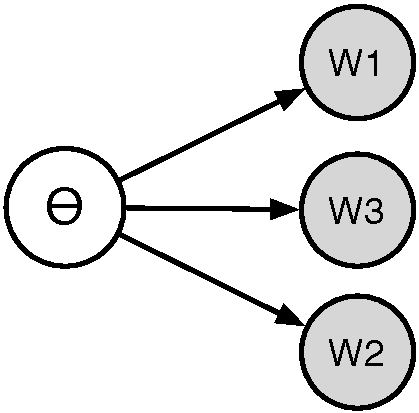
\includegraphics[scale=.9]{pictures/gen}
\end{center}

\end{frame}
\begin{frame}[t]\frametitle{Communication}

To \textsl{communicate} a message $\theta$ -- to inform, persuade, demand, threaten, a producer (the speaker or writer) \textsl{generates} words of different kinds in different quantities


\begin{center}
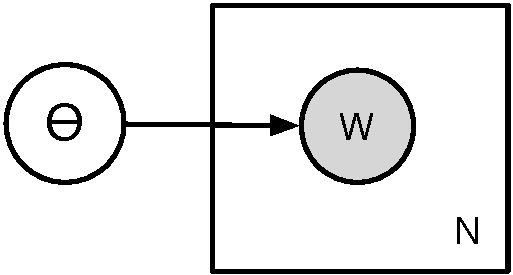
\includegraphics[scale=.9]{pictures/gen-plate}
\end{center}


\end{frame}
\begin{frame}[t]\frametitle{Communication}

To \textsl{understand} a message the consumer (the hearer, reader, coder) uses those words to \textsl{reconstruct} the message

\begin{center}
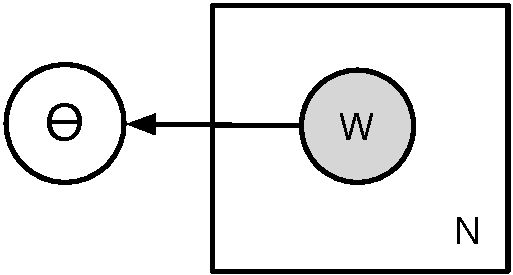
\includegraphics[scale=.9]{pictures/inf-plate}
\end{center}



\end{frame}
\begin{frame}[t]\frametitle{Communication}

This is a stable (Searle, 1995) institutionally conventionalised (Lewis, 1969) but disruptable (Riker, 1996) communication process
in which no finite set of words \textsl{uniquely} identifies any content (Quine, 1960; Davidson, 1977)

How to model this without having to solve the problems of linguistics (psychology, politics) first?

Rely on: instrumentality, conventionalisation, randomness and reflexivity

\end{frame}
\begin{frame}[t]\frametitle{Instrumentality}

Language use is as a \textit{form of action} (Wittgenstein, 1953; Austin, 1975; Dawkins and Krebs, 1978)

Note the distinction between
\ita
\itm `$W$ {means} $X$'
\itm ~~~~~versus
\itm `$W$ {is used to mean} $X$'
\itz

Content analyses to work better when language usage is \textit{stable} and \textit{instrumental}\ldots


%%%% A few words about words

\end{frame}
\begin{frame}[t]\frametitle{Randomness}

\textit{You} know the content of your beliefs (probably)
but others only infer them, on the basis of data
\ita
\itm c.f. `How do I know what I think until I hear what I say?' (E. M. Forster)
\itz
The \textsl{primary data} are often the words you use

You almost never \textit{say exactly the same words twice}, even when you haven't changed your mind.  Hence words are the result of some kind of \textsl{sampling process}.

We treat this process as \textsl{random} because we don't know or care about all the causes of variation
\ita
\itm (and because we're all secretly Bayesians)
\itz

%\slide{Words as Data}
%
%For most methods this is the word frequency matrix
%\begin{align*}
%1.& ~~[W_1, W_2, W_3,\ldots, W_V, \textcolor{red}{\theta_1}]\\
%\vdots~\, & ~~~~~~~~~~~~~~~~~~~~~~~~~~~~~~~~~~~~\vdots\\
%N.& ~~[W_1, W_2, W_3,\ldots, W_V, \textcolor{red}{\theta_N}]
%\end{align*}
%
%We count V words in N documents and try to learn about the content $\theta$
%
%\slide{Hopey Changey Stuff}
%

\end{frame}
\begin{frame}[t]\frametitle{Reflexivity}

Politicians are often nice enough to talk as if they really communicate this way

\ita
\itm My theme here has, as it were, four heads. [\ldots] The first is articulated by the word ``opportunity'' [\ldots] the second is expressed by the word ``choice'' [\ldots] the third theme is summed up by the word ``strength'' [and] my fourth theme is expressed well by the word ``renewal''
\itm (M. Thatcher, 1979)
\itz

[2, 7, 2, 8] in 4431 words

\end{frame}
\begin{frame}[t]\frametitle{More Instrumentality}

The secret of quantitative political text analysis:
\ita
\itm we aren't actually interested in words W
\ita
\itm that's for linguists\ldots
\itz
\itm we aren't actually interested in what's in your head $\theta$
\ita
\itm that's for psychologists\ldots
\itz
\itm
\itm \textbf{except} as they help explain things we are interested in.  They are \textit{just data}.
\itz


%\slide{Modeling}
%
%We will make use of formal models of the process from
%\ita
%\itm the computer sciences: via \textsl{information theory} as \textsl{noisy channel model}
%\itm the social sciences: as an application of \textsl{measurement theory}
%\itz
%(and from British children as a game of `Chinese Whispers' a.k.a. Telephone)
%
%~\\
%For data related reasons we actually \textit{have} to do something like this
%

\end{frame}
\begin{frame}[t]\frametitle{Words as Data}
\begin{center}
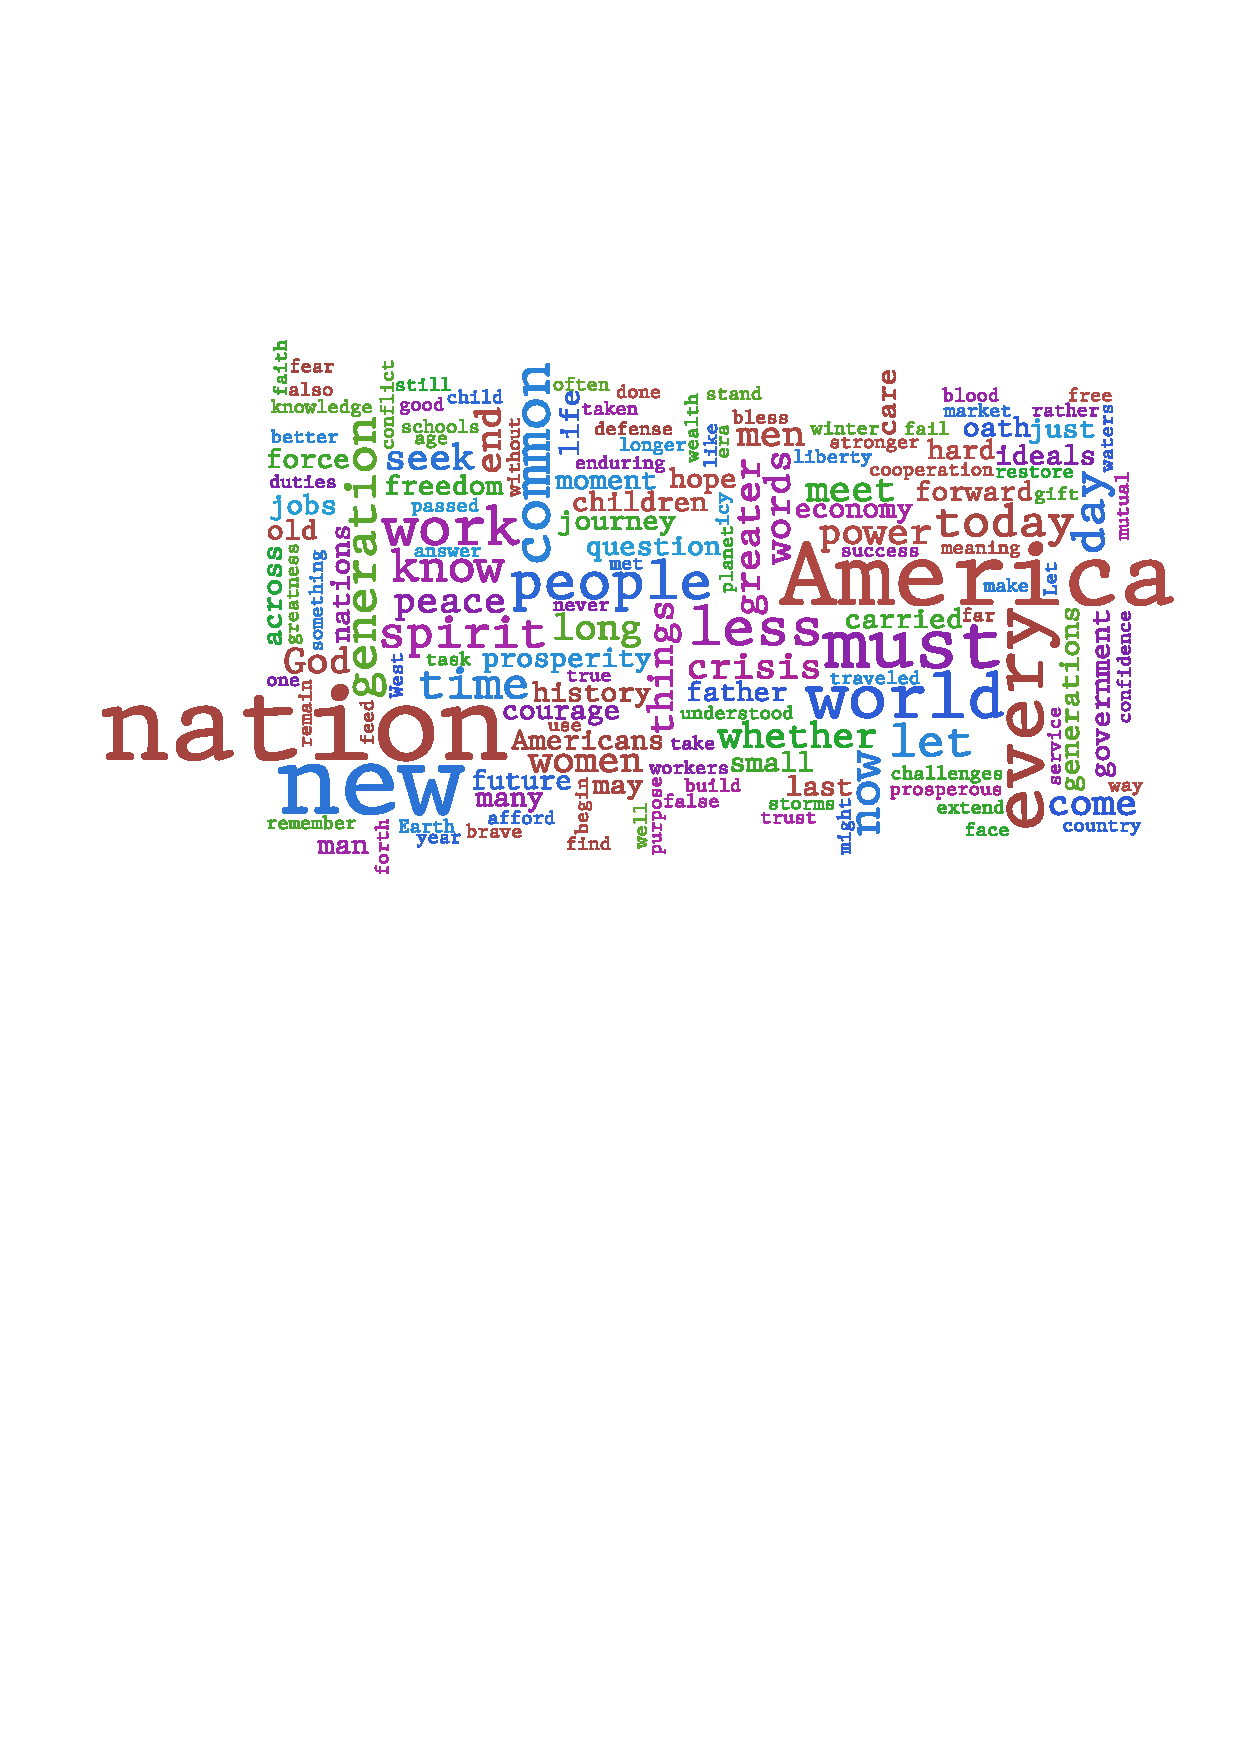
\includegraphics[scale=1.2]{pictures/obamawordle}
\end{center}


\end{frame}
\begin{frame}[t]\frametitle{Words as Data}

What do we know about words \textit{as data}?

They are \textit{difficult}
\ita
\itm High dimensional
\itm Sparsely distributed (with skew)
\itm Not equally informative
\itz


\end{frame}
\begin{frame}[t]\frametitle{Difficult Words}

Example: Labour party (2010) manifesto compared to other parties in two elections\\
~\\
\begin{tabular}{ll}
High D. & 6343 word types in three manifestos \\
Sparse & Of these, Labour only uses 3675 (58\%)\\
Skewed &  Of these 1783 (49\%) words appear exactly once,\\
&  and 2854 (78\%) appear <5 times
\end{tabular}

Average (non-academic) adult vocabulary contains about 10,000 words

Labour manifesto uses about 37\% of commonly available types

%\ite Need substantively-motivated exchangeability assumptions to get a grip

%\ite Stemming / lemmatization helps\ldots a bit\\
%\begin{tabular}{lrl}
%High dimensional & 7154 &$\longrightarrow$ 4642 \\
%Sparse & 2923 (41\%) &$\longrightarrow$ 2120 (46\%)\\
%Skewed & 1436 (49\%) &$\longrightarrow$ 878 (19\%)\\
% & 2420 (83\%) &$\longrightarrow$ 1594 (34\%)
%\end{tabular}

\end{frame}
\begin{frame}[t]\frametitle{Difficult Words}

Words are not like your other data...

Zipf-Mandelbrot law (a pareto distribution in disguise)
\begin{align*}
P(w_i) \propto 1/{r_i^\alpha}
\end{align*}
where $r_i$ is the frequency \textsl{rank} of word i and $\alpha\approx 1$

Very fat tailed\ldots

\end{frame}
\begin{frame}[t]\frametitle{Zipf's Law}

\begin{center}
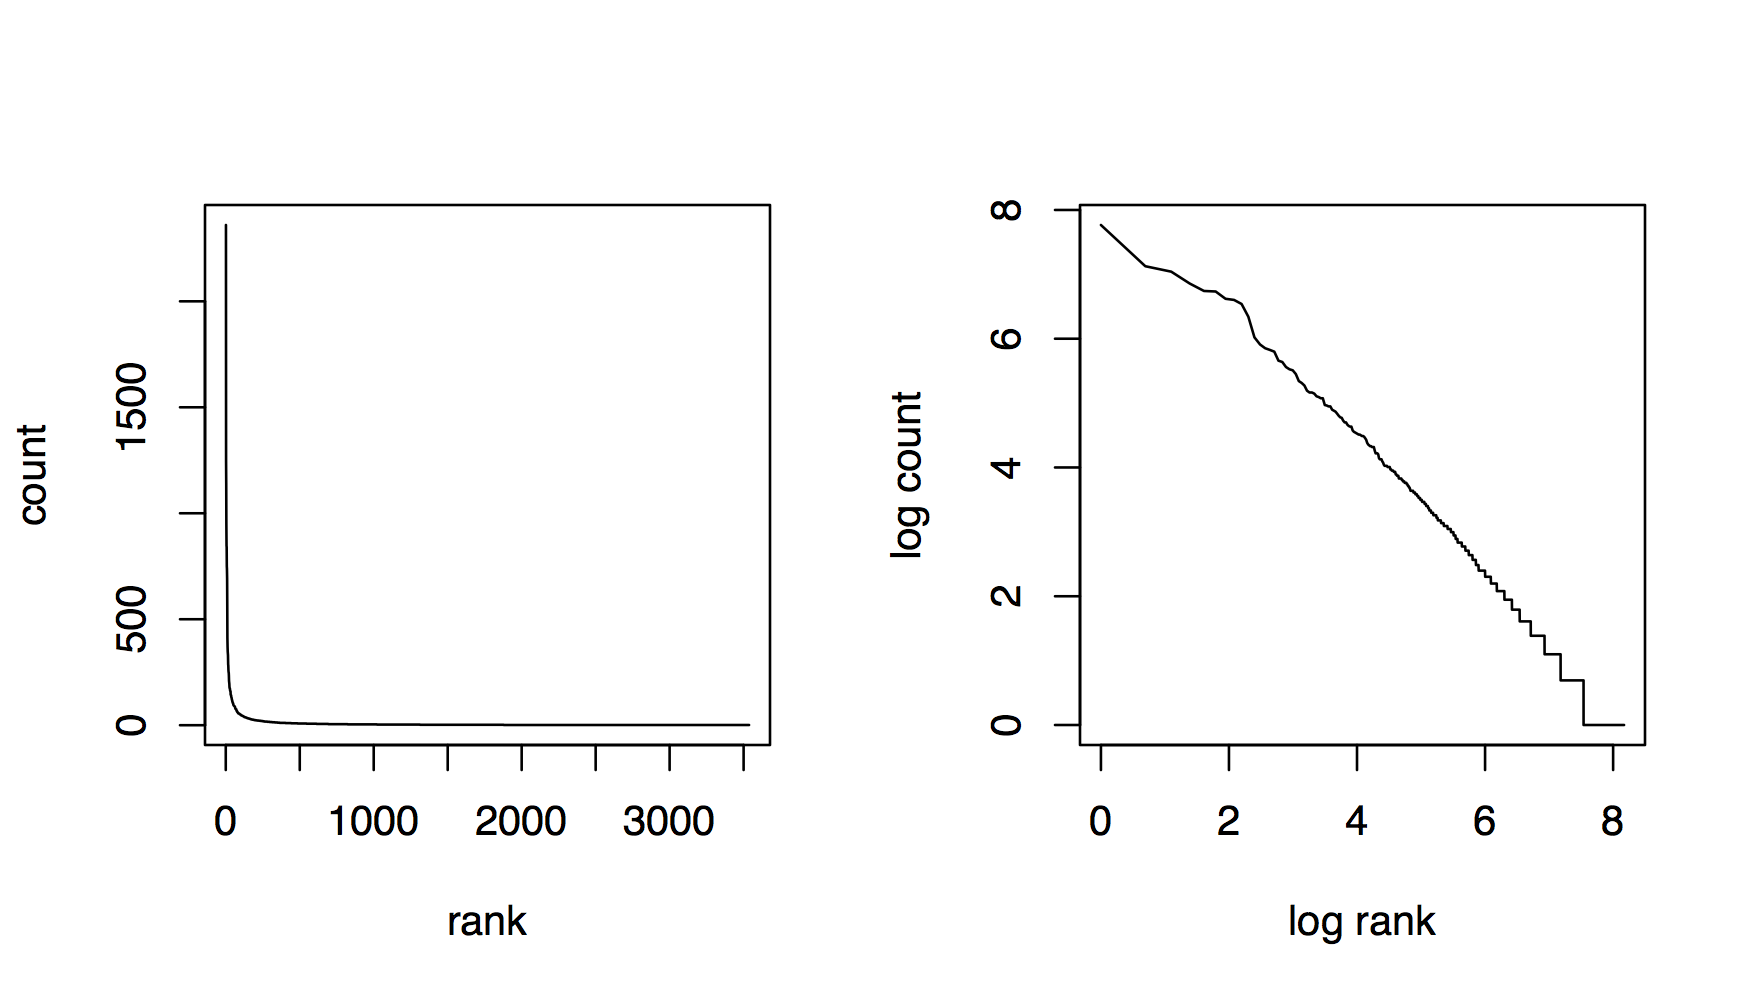
\includegraphics[scale=1.2]{pictures/zipfy}
\end{center}


\end{frame}
\begin{frame}[t]\frametitle{Dealing with Difficult Words}

For large amounts of text summaries are not enough. We need a \textit{model}.

But we need to make some \textsl{exchangeability} assumptions or
\textit{conditional independence} assumptions before we can even do that\ldots

%Two words may
%\begin{tabular}{ll}
%\textsl{refer} to the same thing & (co-reference) \\
%\textsl{mean} the same thing & (synonymy) \\
%are \textsl{adjectives} & (syntactic role)\\
%\textsl{express} hostility, identity, \ldots & (pragmatics)\\
%\end{tabular}

These are typically called the `bag of words'.  Specifically:

\end{frame}
\begin{frame}[t]\frametitle{Text As You Might Read or Hear It}

``As I look ahead I am filled with foreboding.  Like the Roman I seem to see `the river Tiber flowing with much blood'\ldots ''\\
(E. Powell, 1968)


\end{frame}
\begin{frame}[t]\frametitle{Punctuation Invariance}

``As I look ahead I am filled with foreboding.  Like the Roman I seem to see `the river Tiber flowing with much blood'\ldots ''\\
(E. Powell, 1968)
\begin{center}
\small
\begin{tabular}{ll}\toprule
index & token\\ \midrule
1 & as\\
2 & i\\
3 & look\\
4 & ahead\\
5 & i\\
6 & am\\
7 & \ldots\\ \bottomrule
\end{tabular}
~~~~~~~~~~
\begin{tabular}{ll}\toprule
index & token\\ \midrule
1 & like\\
2 & the\\
3 & roman\\
4 & i\\
5 & seem\\
6 & to\\
7 & \ldots\\ \bottomrule
\end{tabular}
\normalsize
\end{center}


\end{frame}
\begin{frame}[t]\frametitle{Lexical Univocality}

\begin{center}
\small
\begin{tabular}{ll}\toprule
type & count\\ \midrule
as & 1\\
i & 2\\
look & 1\\
ahead & 1\\
am & 1\\
\ldots & \ldots\\ \bottomrule
\end{tabular}
~~~~~~~~~~
\begin{tabular}{ll}\toprule
token & count\\ \midrule
like & 1\\
the & 1\\
roman & 1\\
i & 1\\
seem & 1\\
to & 1\\
\ldots & \ldots\\ \bottomrule
\end{tabular}
\normalsize
\end{center}

\end{frame}
\begin{frame}[t]\frametitle{Order invariance}

\begin{center}
\small
\begin{tabular}{rlll}\toprule
&         & unit    & \\ \midrule
&         & `doc' 1 & `doc' 2 \\ \midrule
type      & ahead   & 1    & 0 \\
& am      & 1    & 0 \\
& as      & 1    & 0 \\
& i       & 2    & 1 \\
& like    & 0    & 1\\
& look    & 1    & 0 \\
& roman   & 0    & 1 \\
& seem    & 0    & 1 \\
& the     & 0    & 1 \\
& to      & 0    & 1\\
& \ldots  & \ldots & \ldots \\ \bottomrule
\end{tabular}
\normalsize
\end{center}

\end{frame}
\begin{frame}[t]\frametitle{Count Data}

Yes, we have turned a corpus into a contingency table.

~\\
Everything you learned in your categorical data analysis course applies
\ita
\itm except that some variables of interest: $\theta$ are \textit{not observed}
\itz

%%%%%%%%%%%

\end{frame}
\begin{frame}[t]\frametitle{Down To Business}

\begin{center}
\small
\begin{tabular}{rllllllllll}\toprule
& ahead & am & am & i & like & look &  & \textcolor{gray}{content} \\ \midrule
doc 1  & 1     & 1  & 1  & 2 & 0    & 1    & \ldots & \textcolor{gray}{$\theta_1$} \\
doc 2  & 0     & 0  & 0  & 1 & 1    & 0    & \ldots & \textcolor{gray}{$\theta_2$} \\ \bottomrule
\end{tabular}
\normalsize
\end{center}
~\\\

For each research problem involving content analysis we need to ask:
\ita
\itm What \textit{structure} $\theta$ has
\itm What \textit{modeling strategy} to take
\itm What the \textit{relationship} is between $\theta$ and the words (i.e. the model)
\itz

\end{frame}
\begin{frame}[t]\frametitle{The Structure of $\theta$}

\ita
\itm \textsl{Categorical} structure: topics of newspaper articles or speeches\\Data type: nominal or ordinal (category labels)
\itm \textsl{Dimensional} structure: In spatial politics well-ordered preferences imply distances in an ideological space\\Data type: Real numbers
\itm \textsl{Network} structure: citation analyses, social network analysis\\Data type: nodes and arcs
\itm \textsl{Predicative} structures: assertions about the beliefs of other political actors\\Data type: ??
\itz

\end{frame}
\begin{frame}[t]\frametitle{Statistical Models of Words: Poisson}

Word counts/rates are conditionally Poisson:
\begin{align*}
P(W_j) &~=~ \text{Poisson}(\textcolor{red}{\lambda_{j}})\\
&~=~ \frac{\textcolor{red}{\lambda_{j}}^{W_{j}}~e^{-\textcolor{red}{\lambda}}}{W_{j}!}
\end{align*}

Expected $W_{j}$ (and its variance) is $\lambda_{j}$

Models are mostly proportional because multiplicative
~\\
Conditional on what?  Typically on $\theta$

\end{frame}
\begin{frame}[t]\frametitle{Statistical Models of Words: Poisson}

\centerline{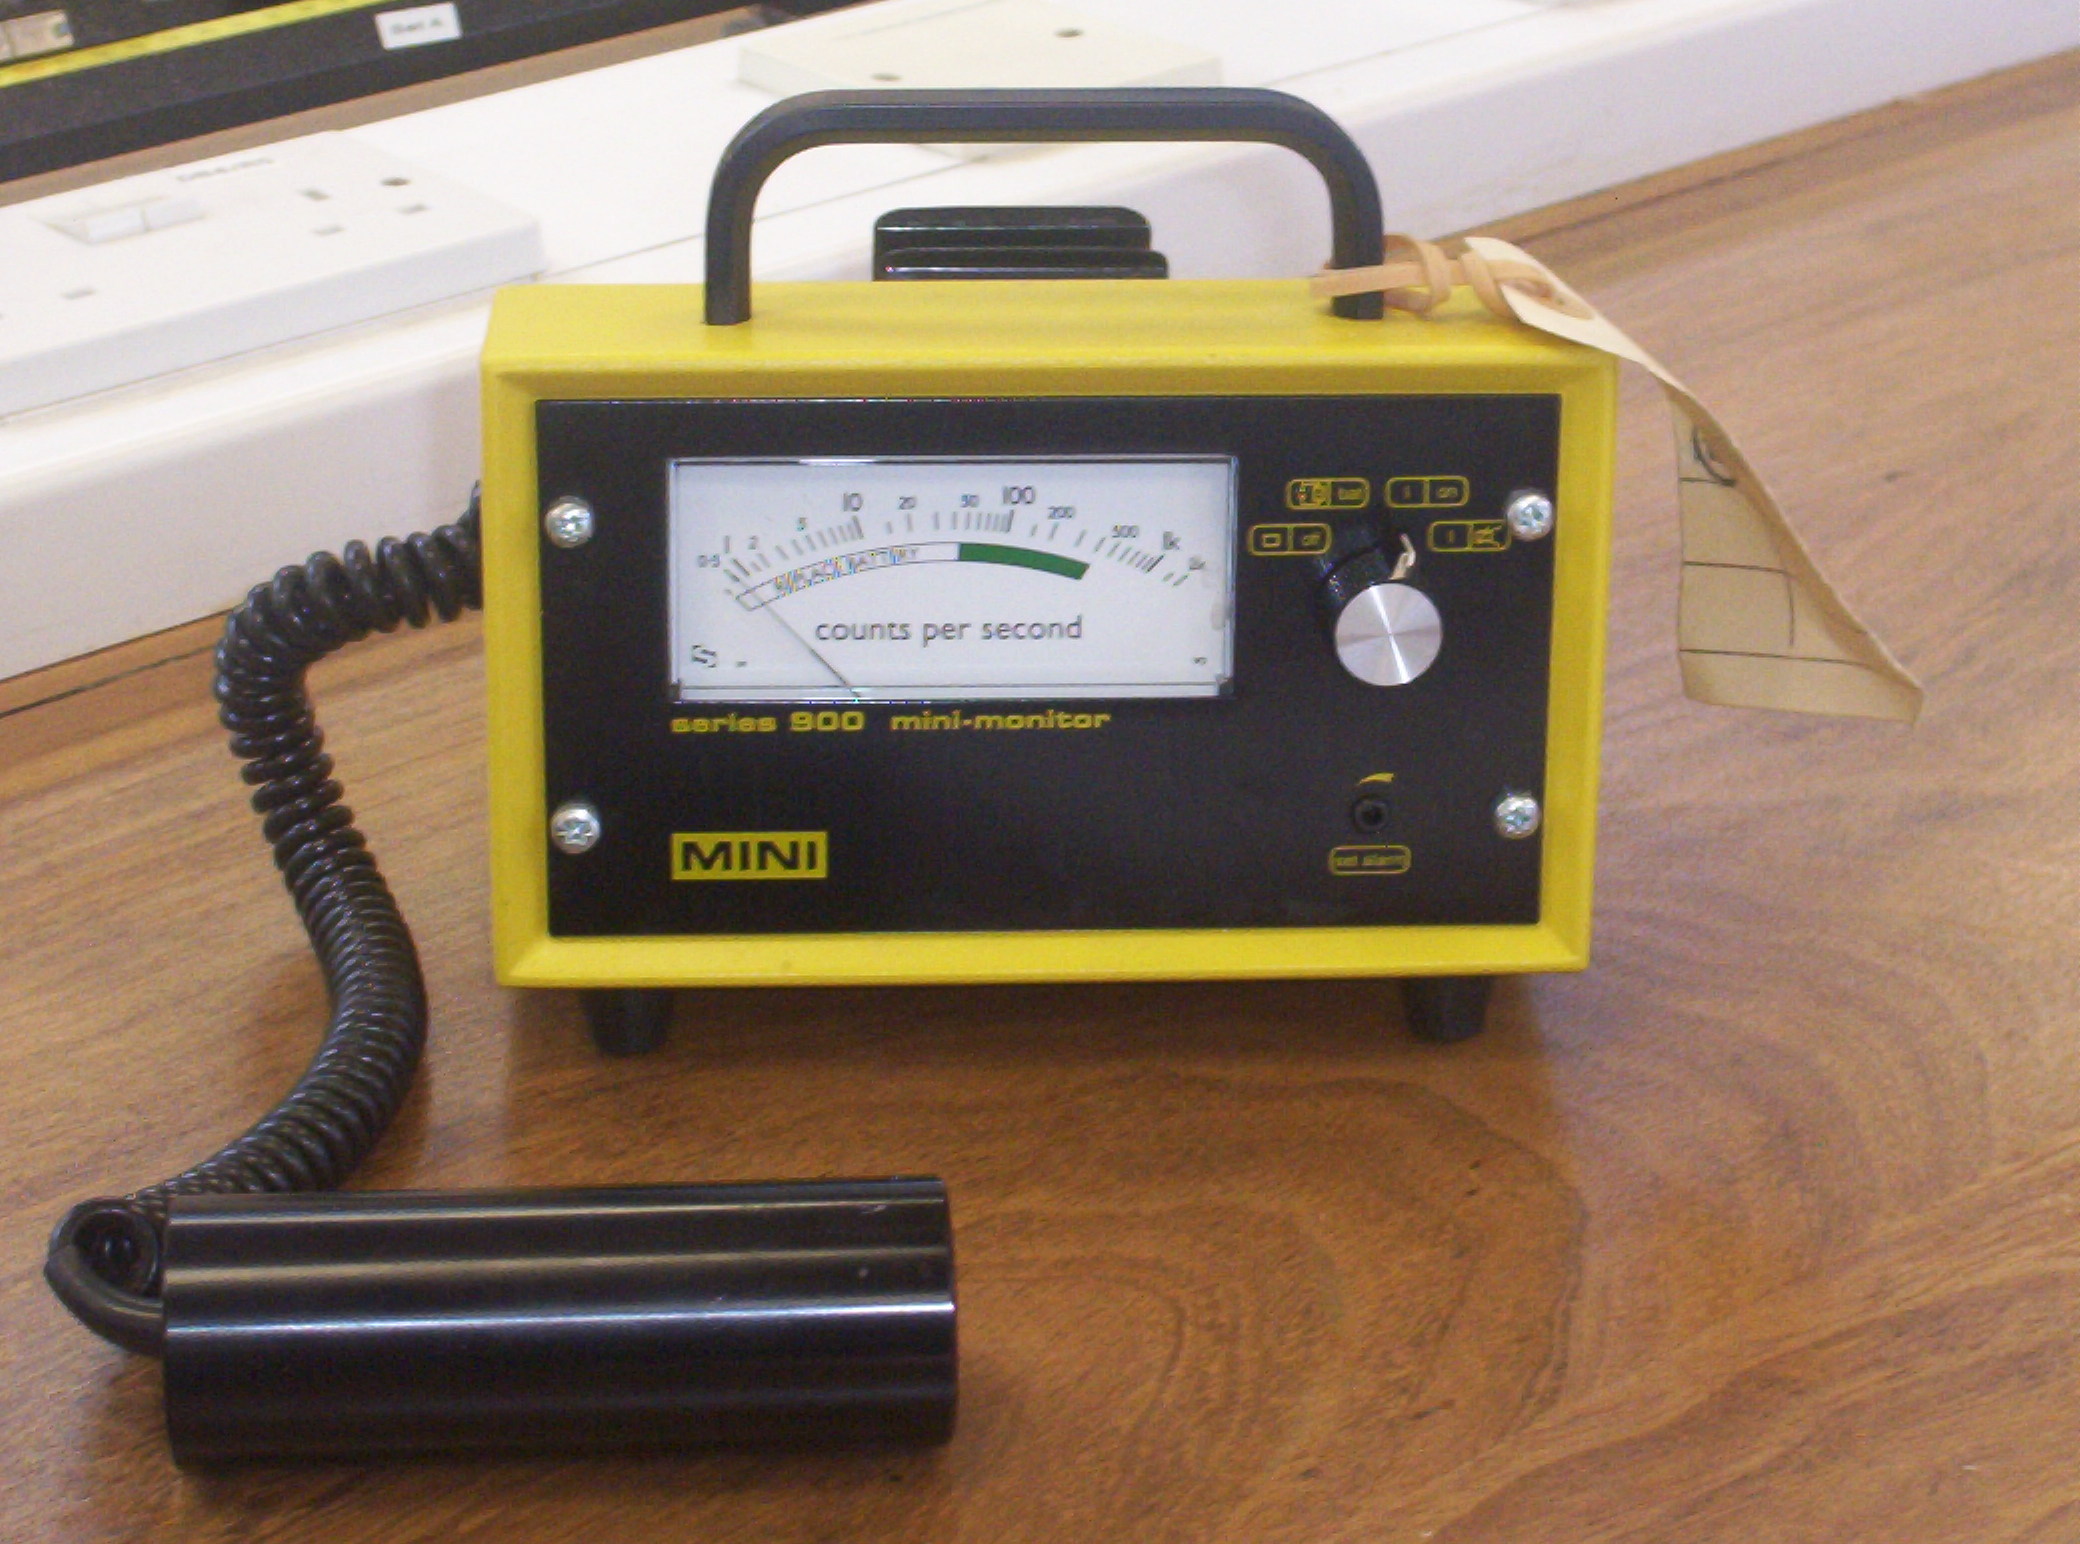
\includegraphics[scale=.2]{pictures/geiger_counter}}

\end{frame}
\begin{frame}[t]\frametitle{Statistical Models of Words: Poisson}

These models are going to think of content as anything that systematically alters word and topic rates


\end{frame}
\begin{frame}[t]\frametitle{Statistical Models of Words: Multinomial}

For fixed document length counts are conditionally Multinomial:
\begin{align*}
P(W_{1}\ldots W_{V}) &~=~ \text{Multinomial}(W_{1}\ldots W_{V}; \textcolor{red}{\pi_{1}}\ldots\textcolor{red}{\pi_{V}}, N_i)\\
&~~~\frac{N!}{W_{1}!\ldots W_{V}!} \prod^{V}_{j} \textcolor{red}{\pi_{j}}^{W_{j}}
\end{align*}
Expected $W_{i}$ is $N\pi_{i}$

Covariance of $W_{i}$ and $W_{j}$ is $-N \pi_{i}\pi_{j}$ (budget constraint)

\end{frame}
\begin{frame}[t]\frametitle{Statistical Models of Words: Multinomial}

\centerline{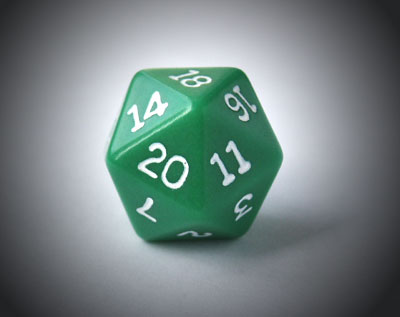
\includegraphics[scale=1]{pictures/20-sided-die}}

\end{frame}
\begin{frame}[t]\frametitle{Statistical Models of Words: Multinomial}

We are going to think about \textit{content topics} as like this

\end{frame}
\begin{frame}[t]\frametitle{We build measurement devices}

\centerline{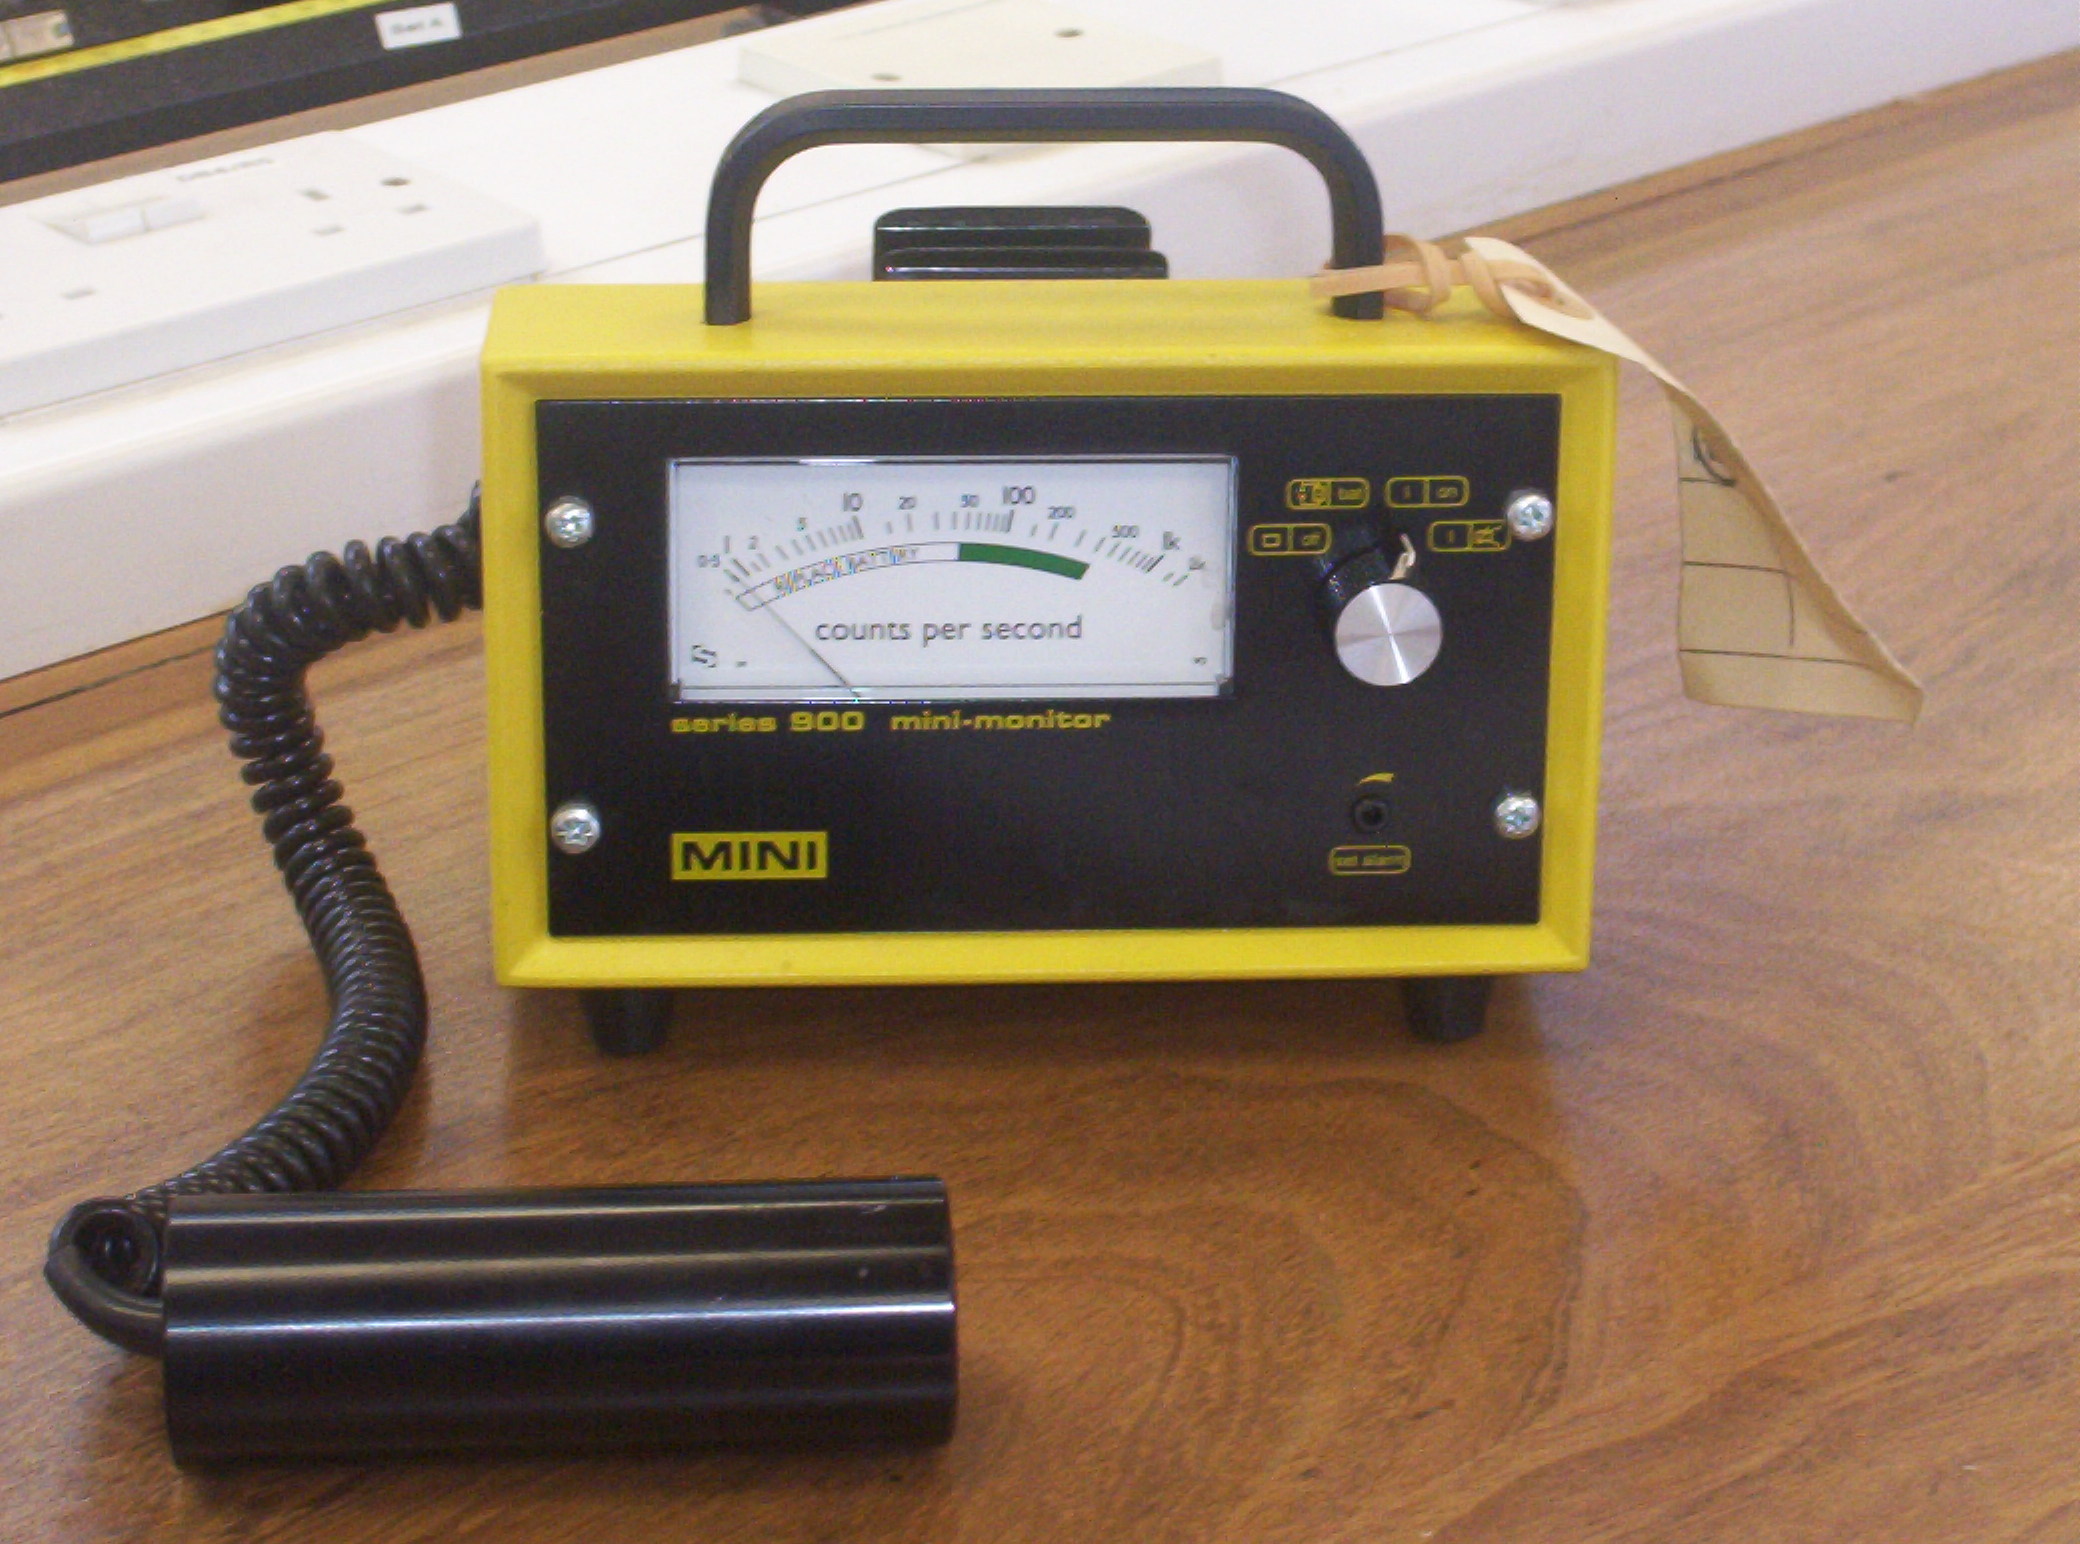
\includegraphics[scale=.2]{pictures/geiger_counter}}

\end{frame}
\begin{frame}[t]\frametitle{(Almost) the big picture}

\centerline{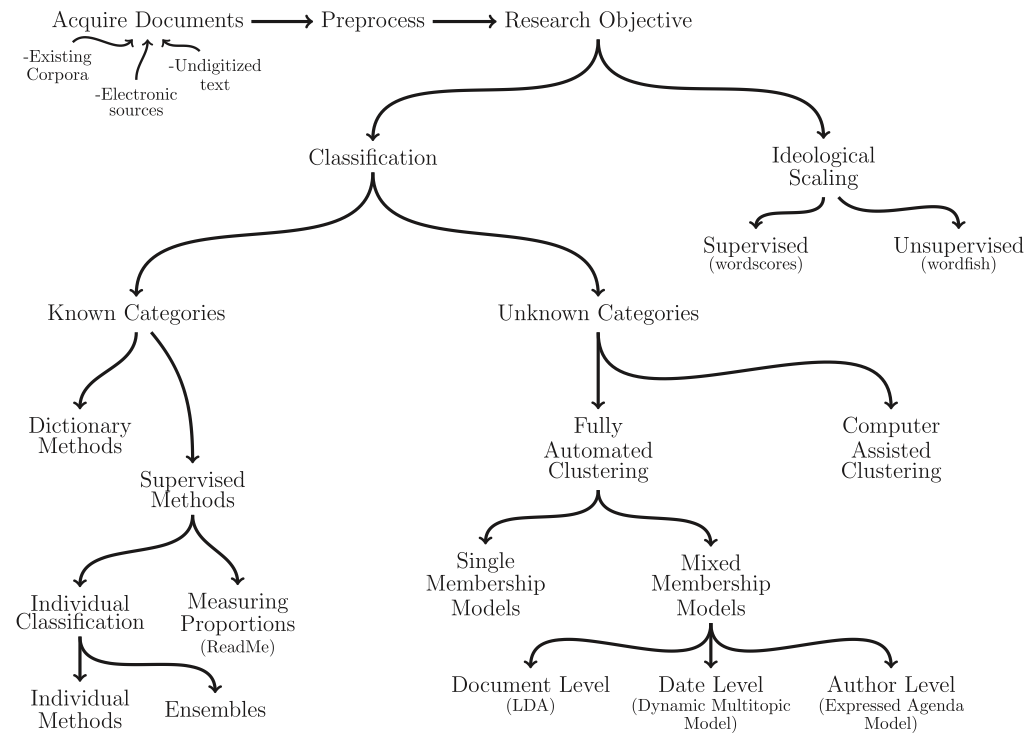
\includegraphics[scale=.5]{pictures/tad-picture}}

\end{frame}
\begin{frame}[t]\frametitle{Really the big picture}

\centerline{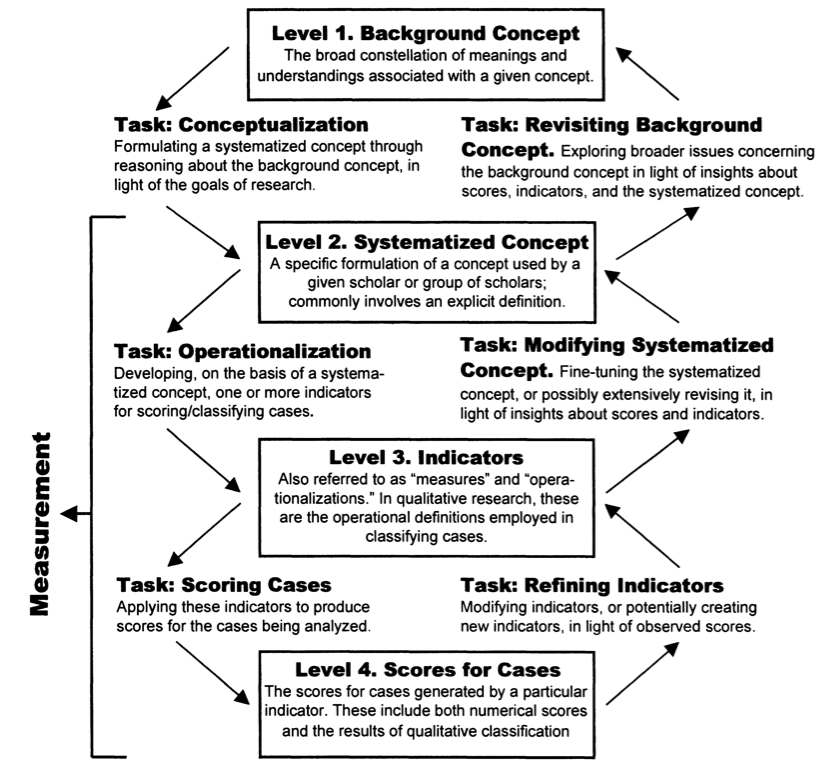
\includegraphics[scale=.45]{pictures/measurement-validity}}

%\slide{Functional form}
%
%What function relates $\theta$ to the words?\\(via the $\lambda$s and $\pi$s)
%
%Depends on the modeling strategy\ldots
%
%Regression / classification style:
%\begin{equation*}
%\theta \Leftarrow W_1 \ldots W_V
%\end{equation*}
%
%Measurement model style:
%\begin{equation*}
%W_1 \ldots W_V \Leftarrow  \theta
%\end{equation*}
%

\end{frame}
\begin{frame}[t]\frametitle{Modeling strategies}

We can model the contents of a word frequency matrix in several ways
\ita
\itm $\theta \longleftarrow \text{words}$: Go for $P(\theta \mid \text{words})$ \textit{directly}
\ita
\itm Requires some \textit{observed} $\theta$, and lots of \textit{careful} regression modeling, or manual coding
\itz
\itm $\theta \longrightarrow \text{words}$: Get $P(\theta \mid \text{words})$ \textit{indirectly}
\ita
\itm Model words as a function of $\theta$, add a prior, and infer $\theta$ using Bayes theorem
\[
P(\theta \mid \text{words}) = \frac{P(\text{words} \mid \theta)P(\theta)}{\sum^\theta_k P(\text{words} \mid \theta_k)P(\theta_k)}
\]
\itz
\itz


\end{frame}
\begin{frame}[t]\frametitle{Modeling Strategies}

These strategies correspond to classification, classical content analysis and topic models, and scaling models

That is to say
\ita
\itm the next three days
\itz

\end{frame}
\begin{frame}[t]\frametitle{Commitment issues}

What are we committing to in this quantitative content analysis framework?

Probably less than you think\ldots

Assumptions:
\ita
\itm $\theta$ is socially / institutionally constructed: only linguists care about the `real' thing
\ita
\itm Note: this does not rule out being objectively correct -- there is a fact about the worth of money in my pocket
\itz
\itm There are no differences in $\theta$ that make no verbal difference (basically Pragmatism)
\itz

\end{frame}
\begin{frame}[t]\frametitle{Absence is an observation}

Don't be fooled\ldots
\ita
\itm Statistical models of text deal with absence as well as presence: zeros count
\itm Absence is informative \textit{to the extent it is surprising}
\itm Surprise implies expectations; expectations imply a model (Kant \textit{and} contemporary neuroscience)
\itz

\newpage

\centerline{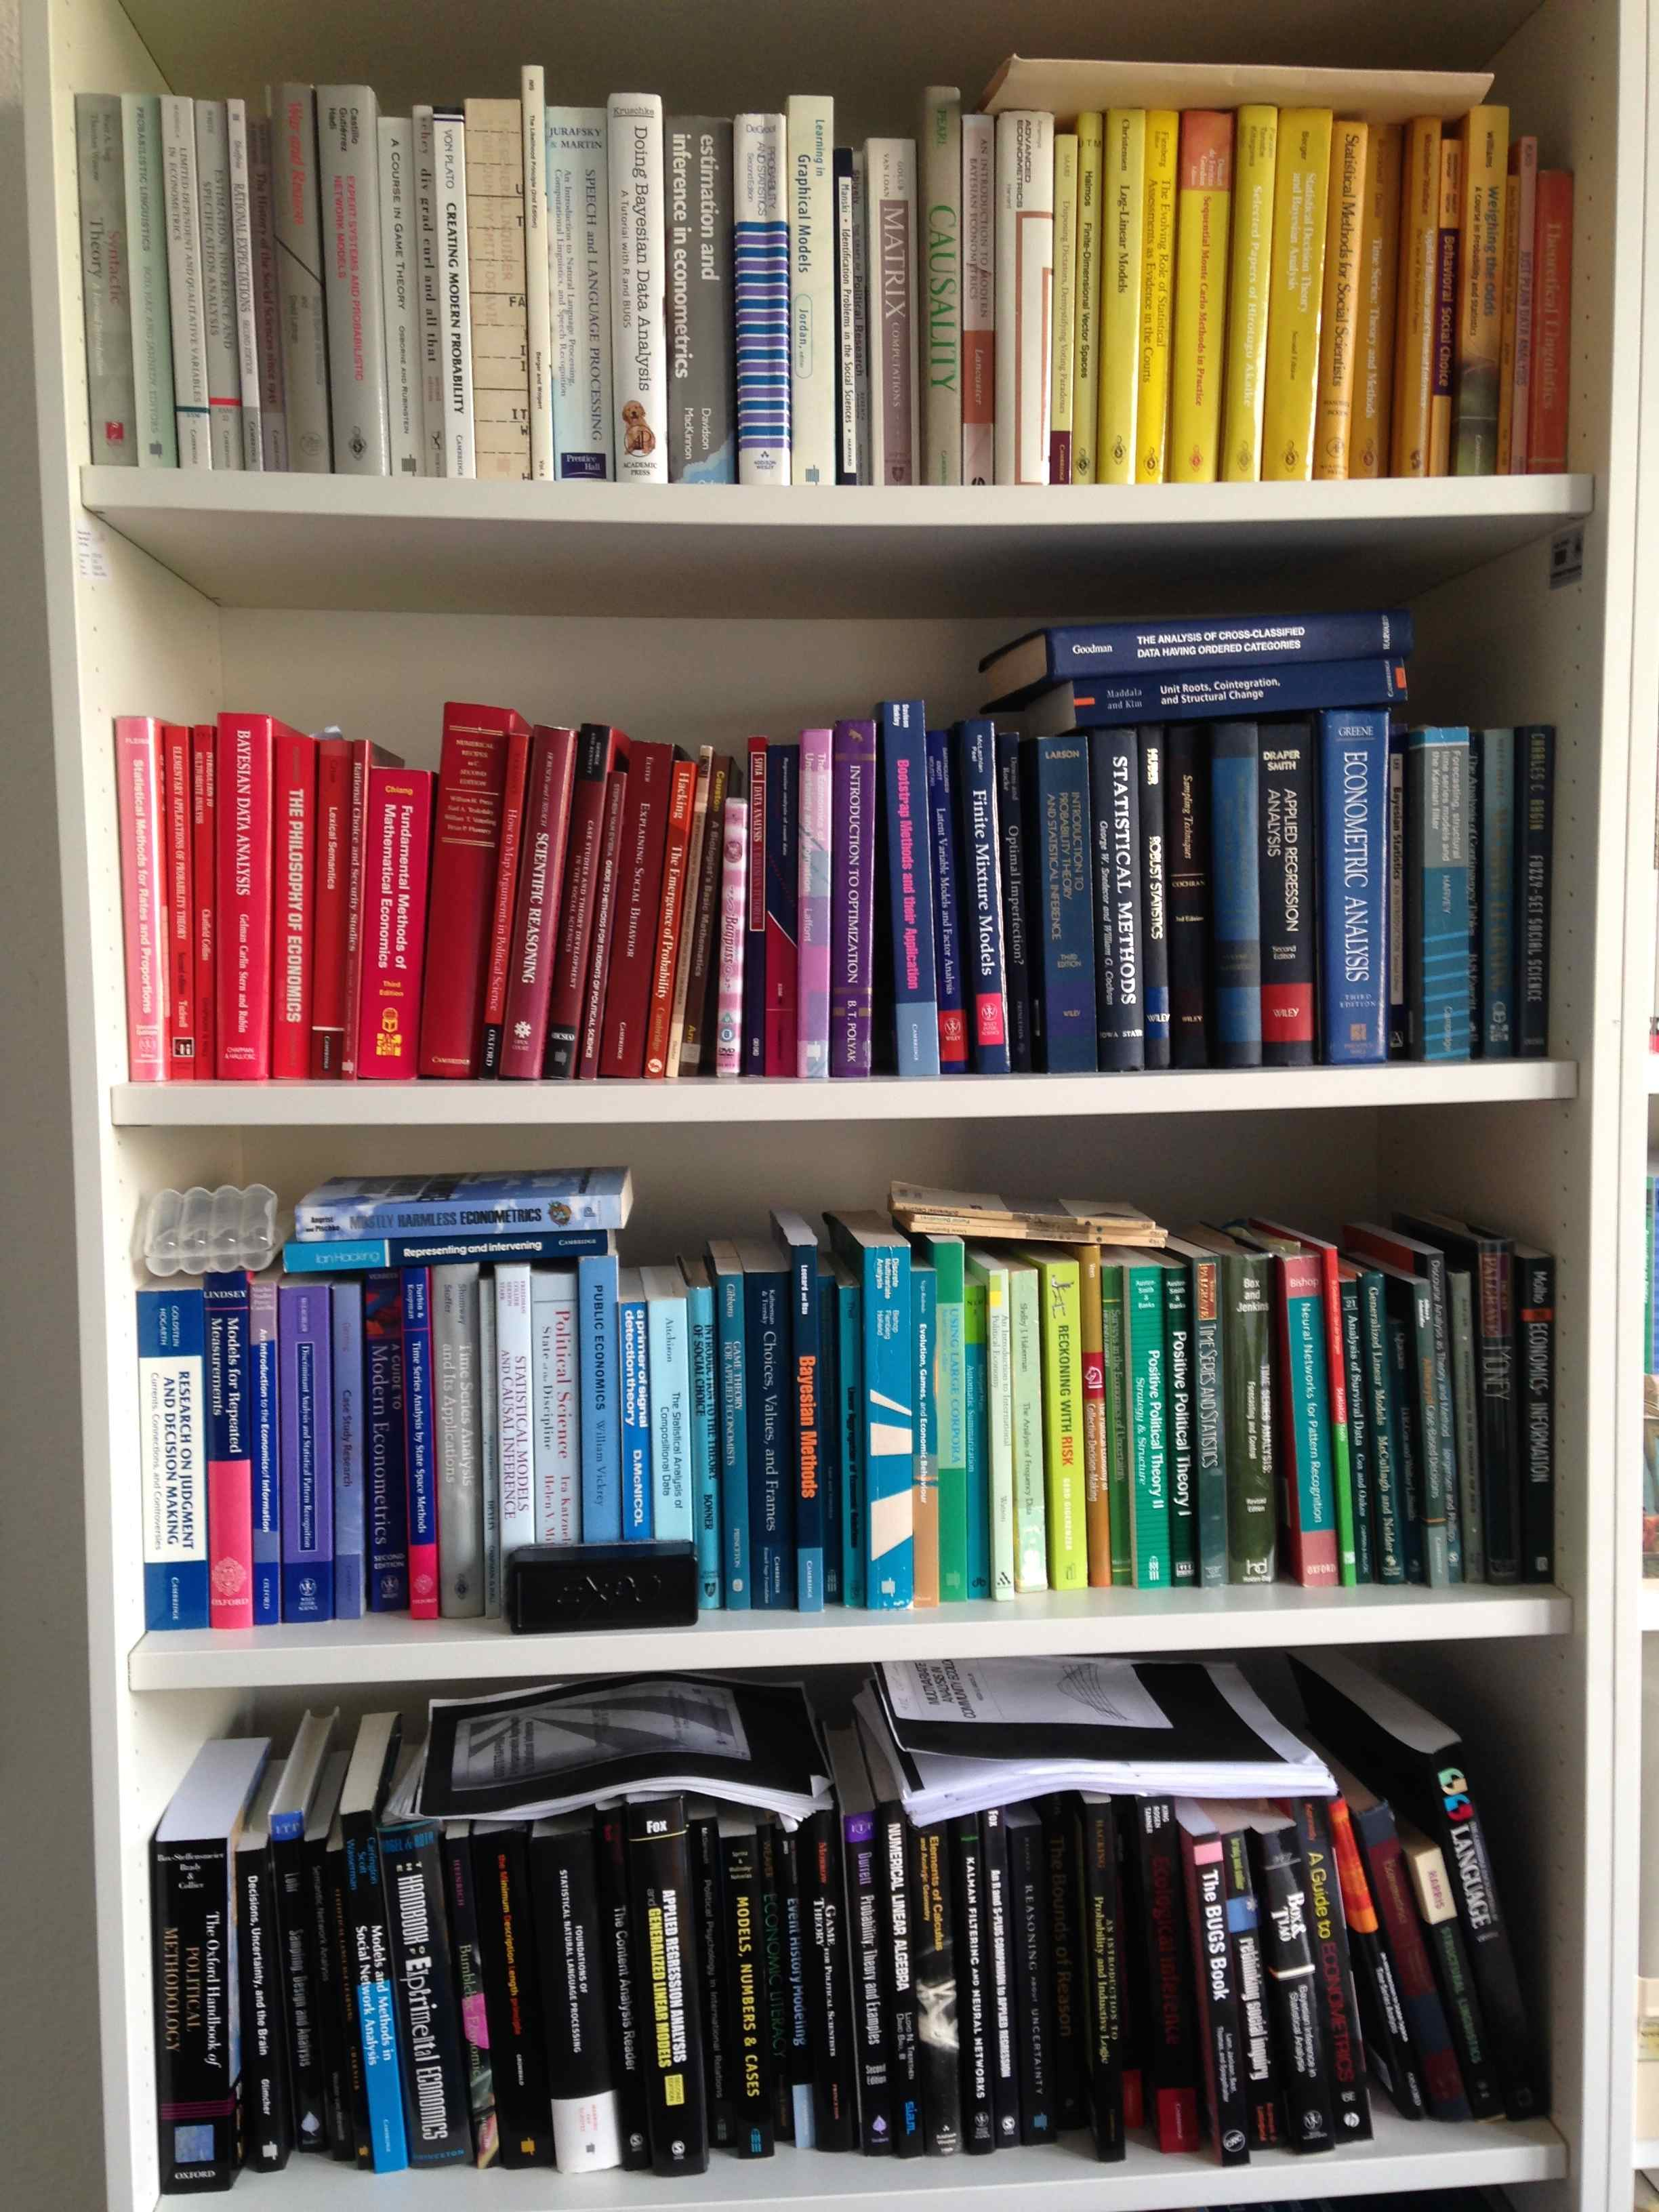
\includegraphics[scale=.12]{pictures/distant-reading}}

\end{frame}
\begin{frame}[t]\frametitle{Theory measurement separation}

Discourse analytic approaches tend to \textit{tightly couple} theory and `measurement' components
\ita
\itm (This is contingent\ldots)
\itz
We will try as far as possible to separate them\ldots
\ita
\itm Our concerns: validity, stability
\itm Can rely on: transparency, reliability, replicability
\itz



\end{frame}
\begin{frame}[t]\frametitle{Menu}

Session 0: How could this possibly work?

Session 1: Dictionary-based `classical' content analysis and topic models
\ita
\itm Content analysis as a model
\itm Applications
\itm Measurement error and how to avoid it
\itm Fun (and trouble) with topic models
\itz

Session 2: Classification and evaluation

Session 3: Scaling Models

%%%%%% CCA here

\end{frame}
\begin{frame}[t]\frametitle{Classical content analysis}

\textsl{Content} is, or is constructed from, \textsl{categories} e.g.
\ita
\itm human rights, welfare state, national security
\itz
Substantively these often have \textsl{valence}, e.g.
\ita
\itm pro-welfare state vs. anti-welfare state, lots of CMP categories
\itz
But they are invariably treated as \textsl{nominal level} variables

We are typically interested in them for
\ita
\itm simple descriptions, making comparisons, tracing temporal dynamics
\itz

\end{frame}
\begin{frame}[t]\frametitle{Talking Like a Newspaper}

\centerline{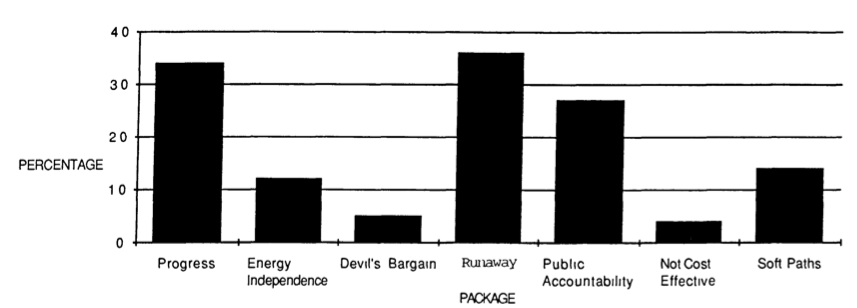
\includegraphics[scale=.8]{pictures/gamson-modigliani-frames-opinion}}
Gamson and Modigliani (1989)


\end{frame}
\begin{frame}[t]\frametitle{Talking like a Candidate}

\centerline{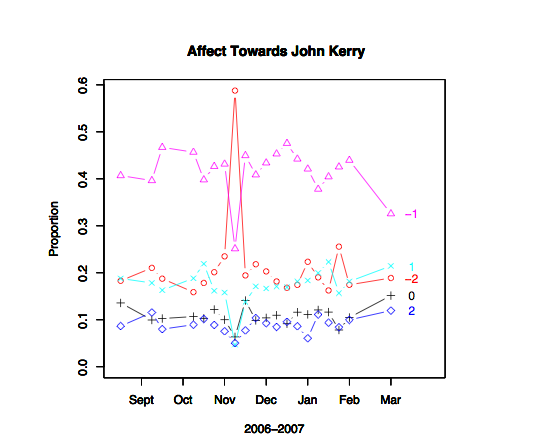
\includegraphics[scale=.7]{pictures/kerry-blogs}}
Hopkins and King (2010)

\end{frame}
\begin{frame}[t]\frametitle{Talking like a Terrorist}

\begin{center}
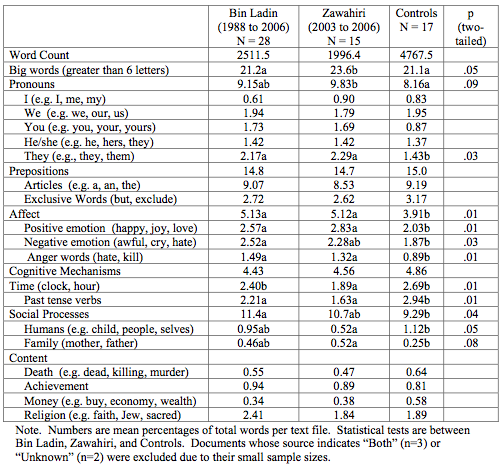
\includegraphics[scale=.7]{pictures/binladen}
\end{center}

\end{frame}
\begin{frame}[t]\frametitle{Talking Like the Commission}

\centerline{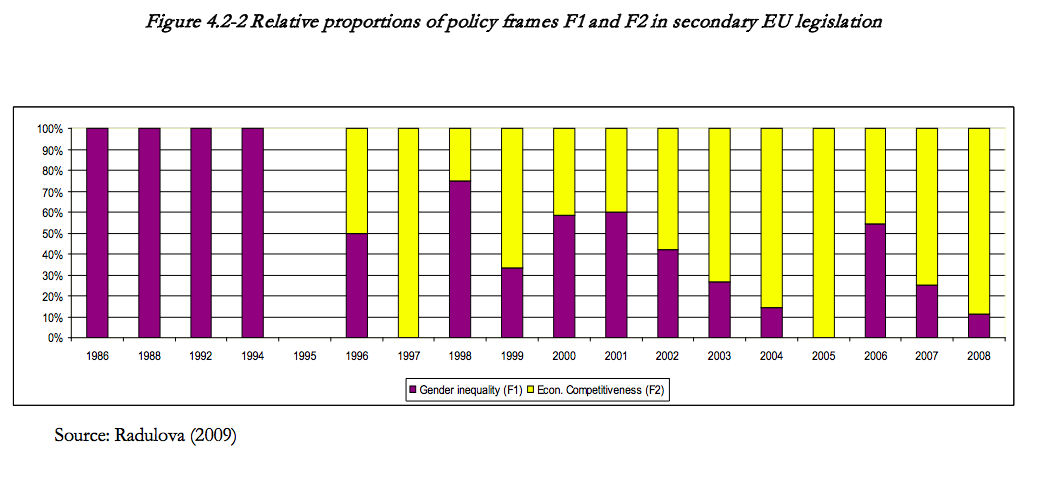
\includegraphics[scale=.75]{pictures/radulova-frames2}}


\end{frame}
\begin{frame}[t]\frametitle{Talking About Drugs}

\centerline{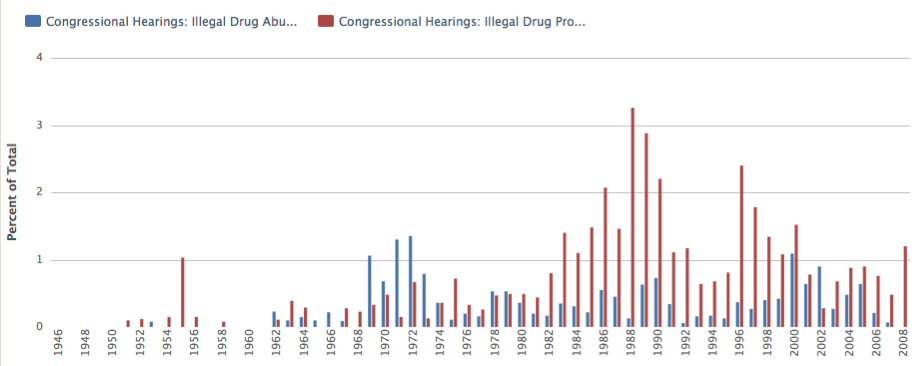
\includegraphics[scale=.75]{pictures/drugs}}

The Congressional Bills Project website (retrieved 2010)
%
%
%\slide{Talking About Drugs}
%
%\centerline{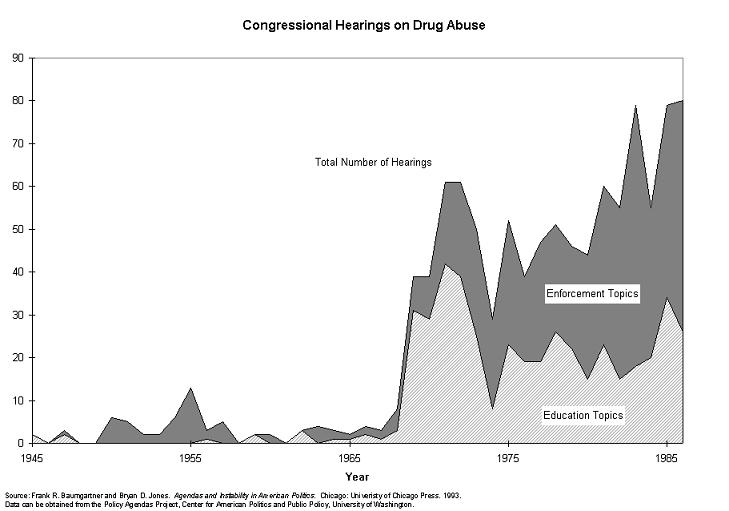
\includegraphics[scale=1]{pictures/policyagendas-drugs-hearings}}

%\slide{Applications: George, Al, and John}
%
%Stump speeches from US presidential candidates in 2000
%
%\slide{Campaigning with negative language}
%\centerline{\includegraphics[scale=.8]{pictures/negative_bar}}
%
%\slide{Campaigning with positive language}
%\centerline{\includegraphics[scale=.8]{pictures/positive_bar}}
%
%\slide{bin Laden, al Zawahiri, and `others'}
%
%\begin{center}
%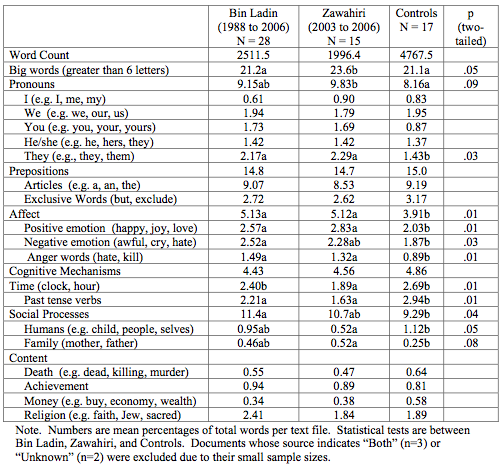
\includegraphics[scale=.8]{pictures/binladen}
%\end{center}
%
%\slide{``and you end up in Iraq''}
%\centerline{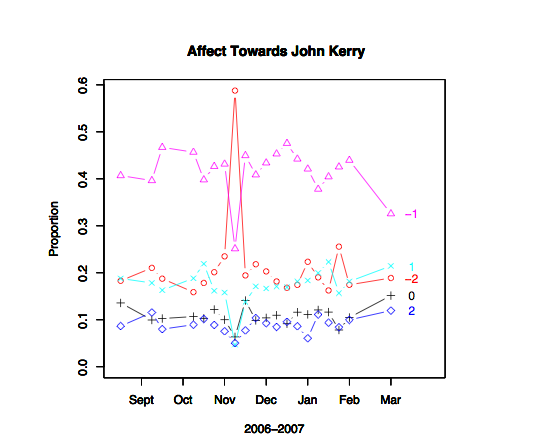
\includegraphics[scale=.8]{pictures/kerry-blogs}}


\end{frame}
\begin{frame}[t]\frametitle{Classical Content Analysis}

Categories are
\ita
\itm equivalence classes over words
\itm representable as assignments of a K-valued category membership variable $Z$ to each word
\itz

~\\
\centerline{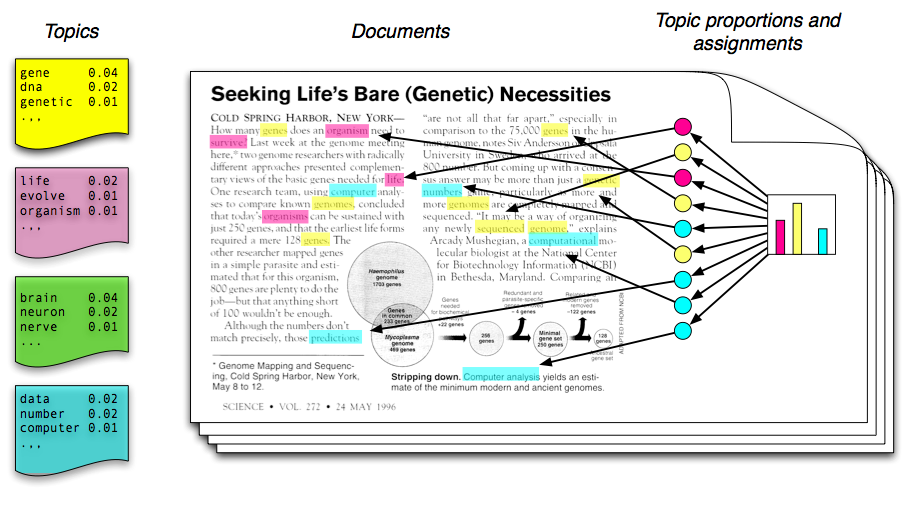
\includegraphics[scale=.6]{pictures/topics2}}


\end{frame}
\begin{frame}[t]\frametitle{Classical Content Analysis}

\centerline{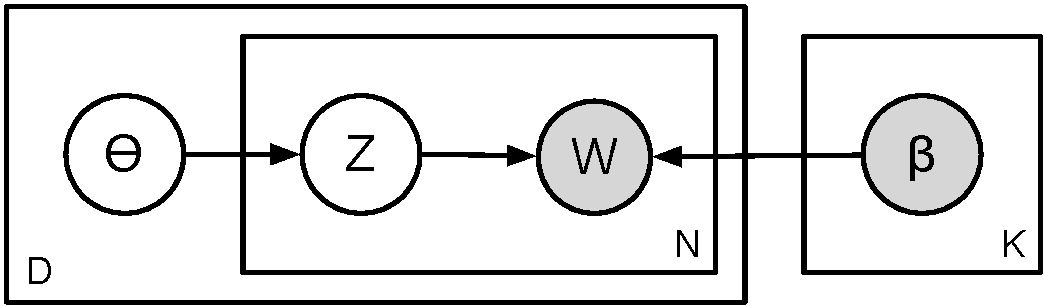
\includegraphics[scale=.9]{pictures/new-topics-ca}}

\end{frame}
\begin{frame}[t]\frametitle{Content Analysis Dictionary}

\small

\begin{tabular}{ll}
ECONOMY & +STATE\\
& accommodation\\
& age\\
& ambulance\\
& assist\\
& \ldots\\
& -STATE\\
& choice*\\
& compet*\\
& constrain*\\
& \ldots
\end{tabular}
\normalsize

from Laver and Garry's (2000) dictionary

\end{frame}
\begin{frame}[t]\frametitle{As a posterior: P(Z | W)}

Translation:  For each word:\\
\begin{center}
\begin{tabular}{lcc} \toprule
& $P(Z=\text{\textsl{state reg}}\mid \text W)$ & $P(Z=\text{\textsl{market econ}} \mid \text W)$ \\ \midrule
\text{age} & 1 & 0 \\
\text{benefit} & 1 & 0 \\
\ldots & \ldots & \ldots\\
\text{assets} & 0 & 1 \\
\text{bid} & 0 & 1\\
\ldots & \ldots & \ldots\\ \bottomrule
\end{tabular}
\end{center}


\end{frame}
\begin{frame}[t]\frametitle{\ldots from a underspecified likelihood: P(W | Z)}

Note that the \textit{only} way this could be true is if
\begin{center}
\begin{tabular}{rcc} \toprule
& \textsl{state reg} & \textsl{market econ} \\ \midrule
$P(\text{age} \mid \text{Z})$ & a & \textbf{0} \\
$P(\text{benefit} \mid \text{Z})$ & b & \textbf{0} \\
\ldots & \ldots & \ldots\\
$P(\text{assets} \mid  \text{Z})$ & \textbf{0} & c \\
$P(\text{bid}  \mid  \text{Z})$& \textbf{0} & d\\
\ldots & \ldots & \ldots\\ \bottomrule
\end{tabular}
\end{center}
where a, b, c, and d > 0
{and} all categories are equally likely: $P(k)=1/K$


\end{frame}
\begin{frame}[t]\frametitle{\ldots leading to a posterior over content}

Define the category \textit{counts}
\begin{align*}
Z_k & = \sum^N_{i} P(Z = k \mid W_i)
\end{align*}
and estimate category relative \textit{proportions} using
\begin{align*}
\hat{\theta}_k &= \frac{Z_k}{\sum^K_{j} Z_j}
\end{align*}

When $\theta$ is a set of multinomial parameters, \textit{and the model assumptions are correct},
this could be a reasonable estimator

\end{frame}
\begin{frame}[t]\frametitle{Reconstruction}

Dictionary-based content analysis was \textit{not} developed this way
\ita
\itm Originally (e.g. Stone 1966) there was no probability model at all
\itz

% Equivalently:
%\ita
%m[] If we know (or can estimate) the parameters $\theta_1,\ldots\theta_{K+1}$ in $P(\theta)$ then we can \textsl{throw away} the word proportions $W_1,\ldots,W_V$
%\itz
% Statistical analogy:
%\ita
%m[] $\theta_1,\ldots\theta_{K+1}$ are sufficient statistics for $W_1,\ldots,W_V$
%\itz


\end{frame}
\begin{frame}[t]\frametitle{Connecting CCA content to politics}

We're usually interested in category proportions per unit (usually document), e.g.
\ita
\itm \textsl{How much} of this document is about national defense?
\itm What is the \textsl{difference} of aggregated left and aggregated right categories (RILE)
\itm How does the \textsl{balance} of human rights and national defense change over time?
\itz


\end{frame}
\begin{frame}[t]\frametitle{Inference About Content}

Statistically speaking, the three types of measures are
\ita
\itm a proportion
\itm a difference of proportions
\itm a ratio of proportions
\itz
Under certain sampling assumptions we can make inferences about a population

%\slide{Inference about proportions}
%
% The large sample standard error for the proportion $\hat{\theta}$ is
%\begin{align*}
%\hat{\sigma} & = \sqrt{\frac{\hat{\theta} (1 - \hat{\theta})}{N}}
%\end{align*}
%where $N$ is the length of the text.  Works better when
%\begin{align*}
%N\hat{\theta}~\text{and}~N(1-\hat{\theta}) > 10
%\end{align*}
% Approximate 95\% confidence interval is
%\begin{align*}
%\hat{\theta} ~\pm~ 1.96 \hat{\sigma}
%\end{align*}

\end{frame}
\begin{frame}[t]\frametitle{Inference About Proportions}

Example: in the 2001 Labour manifesto there are 872 matches to Laver and Garry's \textsl{state reg} category
\ita
\itm 0.029 (nearly 3\%) of the document's words
\itm 0.066 (about 6\%) of words that matched \textsl{any} categories
\itz
The document has 30157 words, so the \textsl{first} proportion is estimated as
\begin{align*}
\hat{\theta}_\text{\textsl{state reg}} & ~=~ 0.029 ~~[0.027, 0.030]
\end{align*}
What does this mean?

\end{frame}
\begin{frame}[t]\frametitle{Inference About Proportions}

Think of the party headquarters repeatedly \textsl{drafting} this manifesto

The true proportion -- the one suitable to the party's policies -- is fixed but every draft is slightly different

The confidence interval reflects the fact that we expect long manifestos to have more precise information about policy

This interval is computed as if every word was a new (conditionally) independent piece of of information

\end{frame}
\begin{frame}[t]\frametitle{Reporting: Rates}

Don't report proportions if you don't need to.

\textsl{Rates/ratios} are more intuitive

e.g. the rate of dictionary matches per $B$ words is
\[
\lambda_B = \theta B
\]
which is a more interpretable proportion,
e.g.
\ita
\itm 29 times per 1000 words
\itz
Different measures correspond to different choices of $B$.

%\slide{Inference about differences}
%
%The large sample standard error for $\hat{\theta}_i - \hat{\theta}_j$ is
%\begin{align*}
%\hat{\sigma} & = \sqrt{\frac{\hat{\theta_i} (1 - \hat{\theta_i})}{N} +
%\frac{\hat{\theta_j} (1 - \hat{\theta_j})}{N}}
%\end{align*}
%where $N$ is the length of the text.  Works better when
%\begin{align*}
%N\hat{\theta}~\text{and}~N(1-\hat{\theta}) > 10
%\end{align*}
%Approximate 95\% confidence interval is
%\begin{align*}
%\hat{\theta}_i-\hat{\theta}_j ~\pm~ 1.96 \hat{\sigma}
%\end{align*}
%
%\slide{Inference About Differences}
%
%UK Conservatives tend to target rural voters.
%
%How much more attention did they get from the Conservatives than from Labour in 2001?
%
%Consider the (very small) category RURAL
%
%Conservatives match 29 words, Labour 31, but Labour's manifesto is longer so
%\begin{align*}
%\hat{\theta}^{\text{LAB}} - \hat{\theta}^{\text{CON}} &~=~ -0.0012 ~~[-0.0003,-0.002]
%\end{align*}
%This difference is significant\ldots

%\slide{Ratios of category proportions}

% Laver and Garry define \textsl{state reg} and \textsl{market econ} categories\\

%\begin{center}
%\begin{tabular}{ll}
%AGED & AUTONOMY\\
%CARE & BUSINESS \\
%DISADVANTAGED & CHOICE* \\
%EXPLOITAT*& CRIPPLING \\
%HUNGER &SHARES \\
%SCHOOLS & HOMESTEAD*\\
%FAIR* & TAX \\
%VULNERABLE & TAX-FREE\\
%WIDOW & THRIFT\\
%\ldots & \ldots
%\end{tabular}
%\end{center}

\end{frame}
\begin{frame}[t]\frametitle{Ratios: How 'New' was New Labour?}

Was the Conservative party in 1992 more or less for state intervention than 'New' Labour in
1997?

Compare instances of \textsl{state reg} and \textsl{market econ} in the manifestos\\
\begin{center}
\begin{tabular}{lllll}\toprule
Party & \multicolumn{2}{l}{Counts}  \\ \midrule
& \textsl{state reg}    &    \textsl{market econ}  \\
Conservative  & 320   & 643 \\
Labour   & 396   & 268      \\ \bottomrule
\end{tabular}
\end{center}

\end{frame}
\begin{frame}[t]\frametitle{Risk Ratios}

Compute two \textsl{risk ratios}:

\begin{align*}
RR_{\text{\textsl{state reg}}} & ~=~ \frac{P(\text{\textsl{state reg}} \mid \text{cons})}
{P(\text{\textsl{state reg}} \mid \text{lab})}\\
RR_{\text{\textsl{market econ}}} & ~=~ \frac{P(\text{\textsl{market econ}} \mid \text{cons})}
{P(\text{\textsl{market econ}} \mid \text{lab})}
\end{align*}
and 95\% confidence intervals

%\slide{Risk Ratios}
%
%
%Standard error around estimated log $RR$ is
%\begin{align*}
%\hat{\sigma} &=  \sqrt{\frac{1}{Z_\text{cons}}-\frac{1}{N_\text{cons}}+\frac{1}{Z_\text{lab}}-\frac{1}{N_\text{lab}}}
%\end{align*}
%95\% Confidence interval around log $RR$ is
%\begin{align*}
%\text{log}\,RR ~\pm~ 1.96 \hat{\sigma}
%\end{align*}
%Exponentiate the estimate and endpoints to get an interval for the risk ratio
%
\end{frame}
\begin{frame}[t]\frametitle{Interpreting Risk Ratios}

If $RR=1$ then the category occurs at the same rate in labour and conservative manifestos

If $RR=2$ then the conservative manifesto contains \textsl{twice} as much \textsl{state reg} language as the labour manifesto

If $RR=.5$ then the conservative manifesto contains \textsl{half} as much \textsl{state reg} language as the labour manifesto

If the confidence interval for $RR$ contains 1 then we \textsl{no evidence} that \textsl{state reg} and \textsl{market econ} occur at different rates

\end{frame}
\begin{frame}[t]\frametitle{Risk Ratios}
\begin{center}
\begin{tabular}{rl} \toprule
& Risk Ratio\\ \midrule
\textsl{market econ} & 1.45 [1.26, 1.67]\\
\textsl{state reg} & 0.49 [0.42, 0.57] \\ \bottomrule
\end{tabular}
\end{center}

Conservative manifesto generates \textsl{market econ} words 45\% more often
\ita
\itm 45\% = 100(1.45 - 1)\%
\itz
Conservative manifesto only generates 49\% as many \textsl{state reg} words as Labour.

Equivalently Labour generates them about \textsl{twice} as often

\end{frame}
\begin{frame}[t]\frametitle{Extensions: Regularised log odds}

\centerline{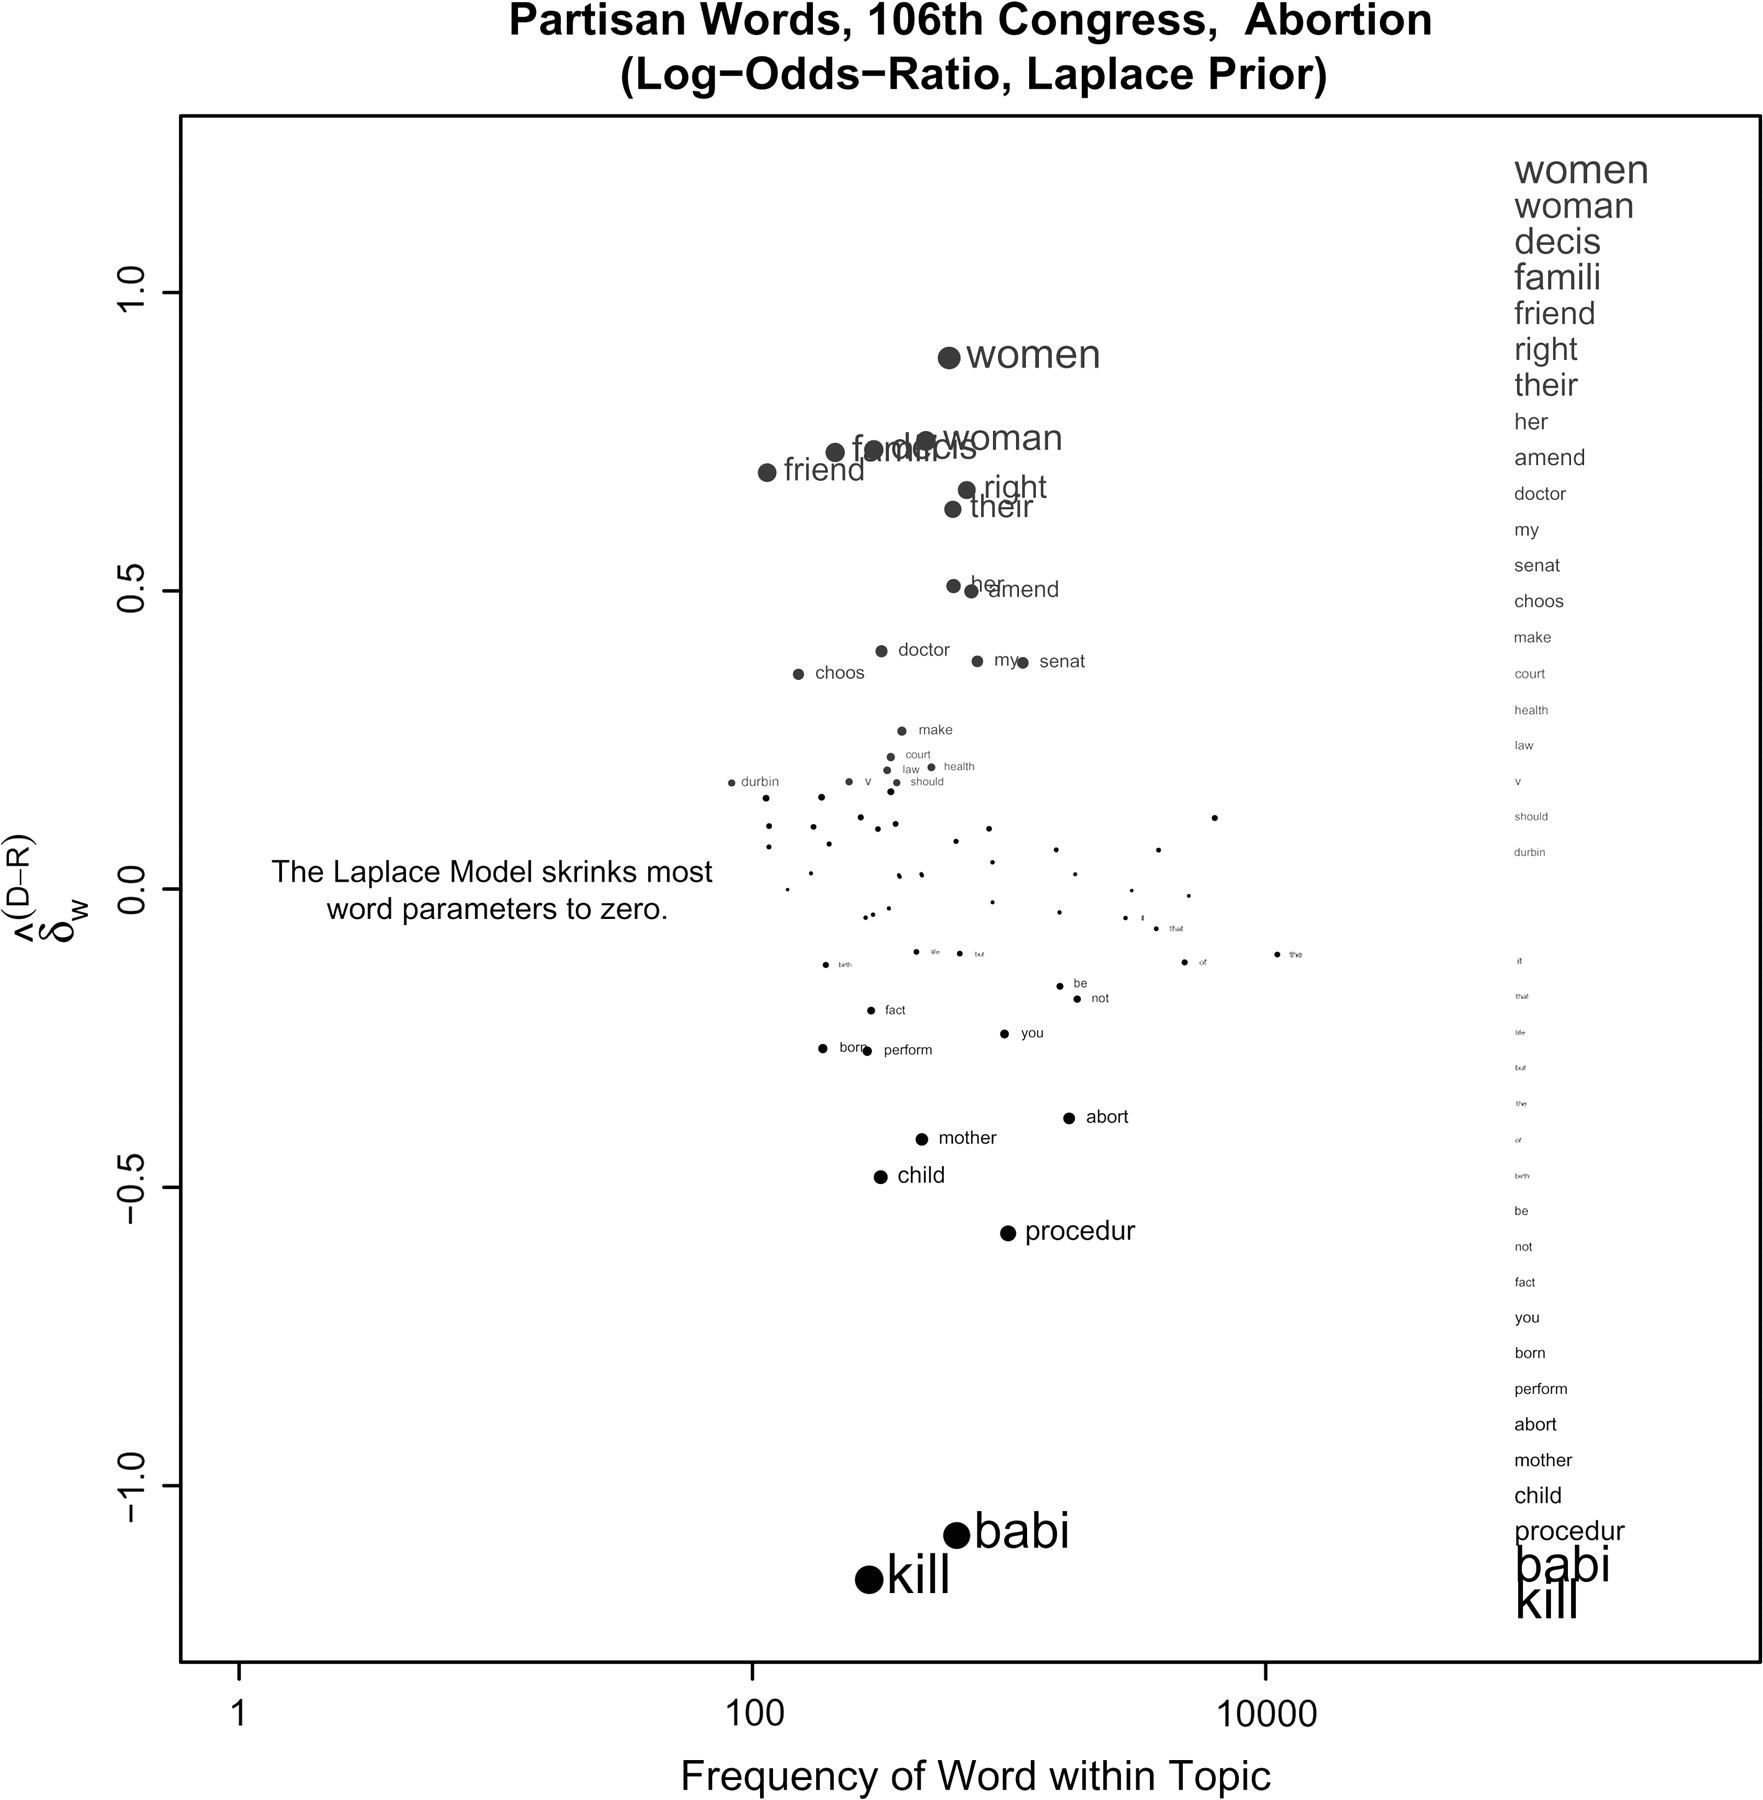
\includegraphics[scale=.2]{pictures/fightin1}}



%\slide{What not to do with counts: Drugs policy}

%\centerline{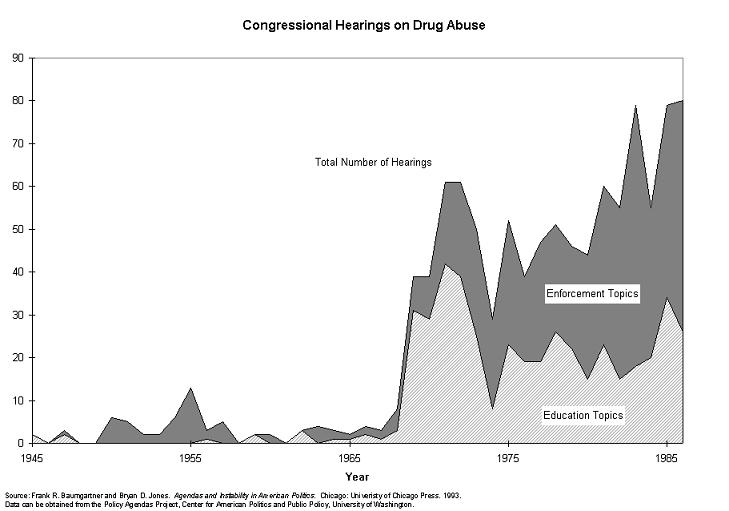
\includegraphics[scale=.8]{pictures/policyagendas-drugs-hearings}}

\end{frame}
\begin{frame}[t]\frametitle{\ldots as dependent variable}

Example: district vs party focus

~\\
\centerline{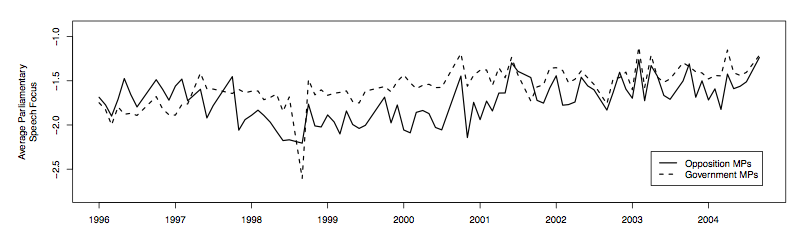
\includegraphics[scale=.8]{pictures/district-party-focus}}

Data: [\textsl{district words}, \textsl{party words}] (Kellerman \& Proksch, MS)

Here, a \textit{logged ratio} of two categories

\end{frame}
\begin{frame}[t]\frametitle{Content as something to explain (Sullivan and Lowe 2007)}

\centerline{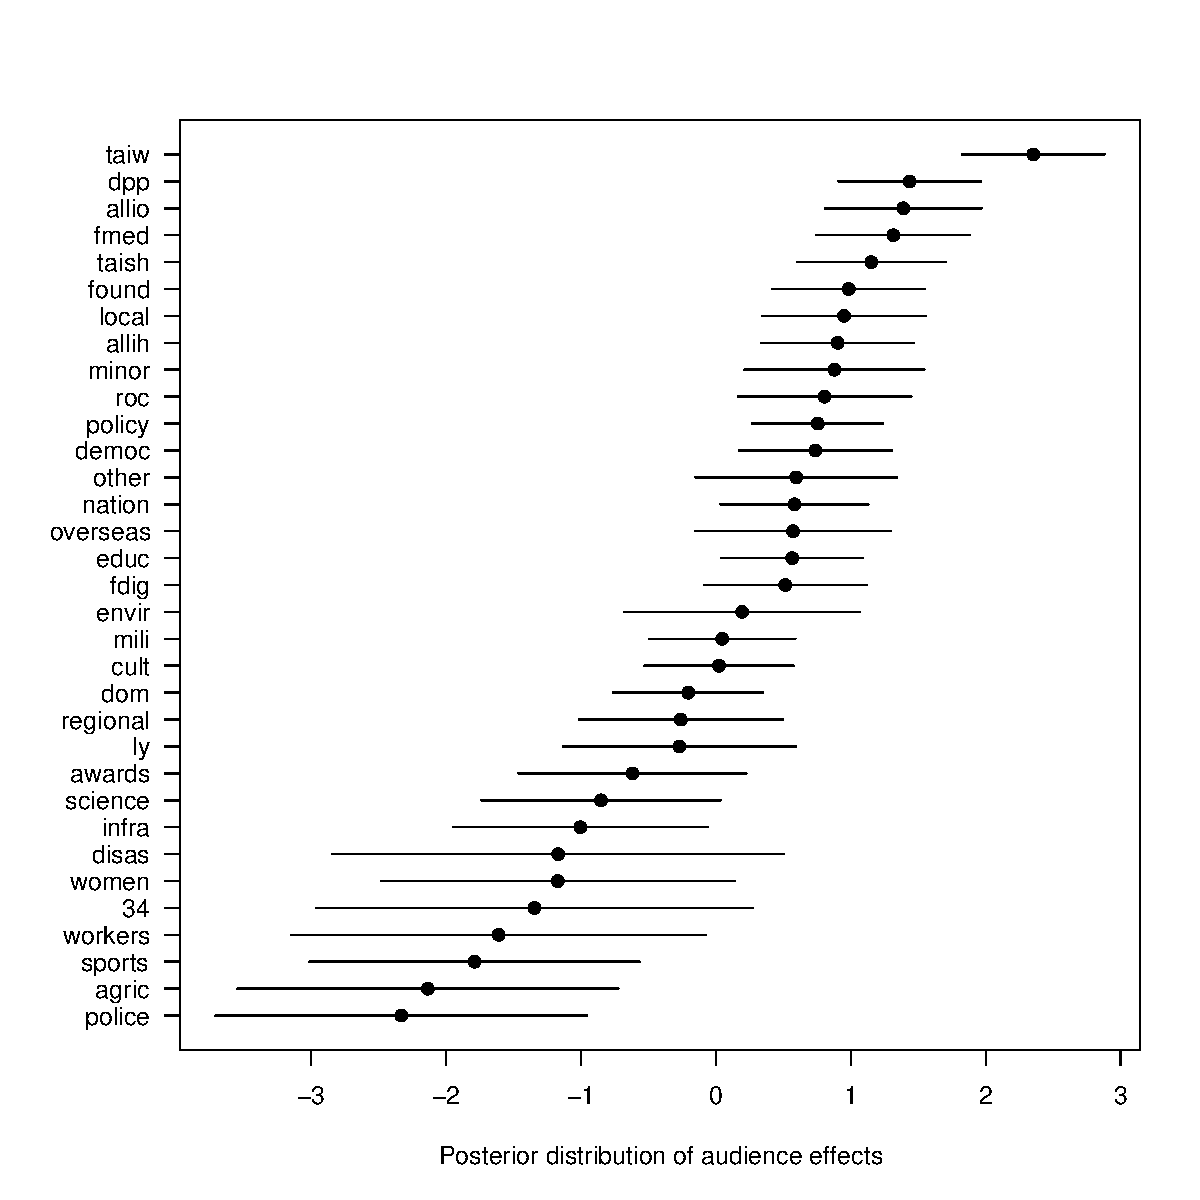
\includegraphics[scale=.5]{pictures/indep-ref}}

\textsl{independence words} $\leftarrow$ audience + offset(doc length)

\end{frame}
\begin{frame}[t]\frametitle{What to report?}

Not all choices are constant or comparable\ldots

{\small
\begin{center}
\begin{tabular}{ll} \toprule
Quantity & Comparability\\ \midrule
Count & No \\
Proportion of words & Yes\\
Proportion of category matches & Yes\\
Rate per B words & Yes\\
Rate per sentence / paragraph & No\\
Difference of proportions & Yes\\
(Logged) ratio of counts & Yes\\
Significance of tests & No!\\
\bottomrule
\end{tabular}
\end{center}
\normalsize}

(if length is uninformative \& category probability constant)


\end{frame}
\begin{frame}[t]\frametitle{OK, how do I make such an instrument?}

Maximise measurement validity

Minimise \textsl{measurement error}

~\\
(Sell high, buy low)
\newpage
\centerline{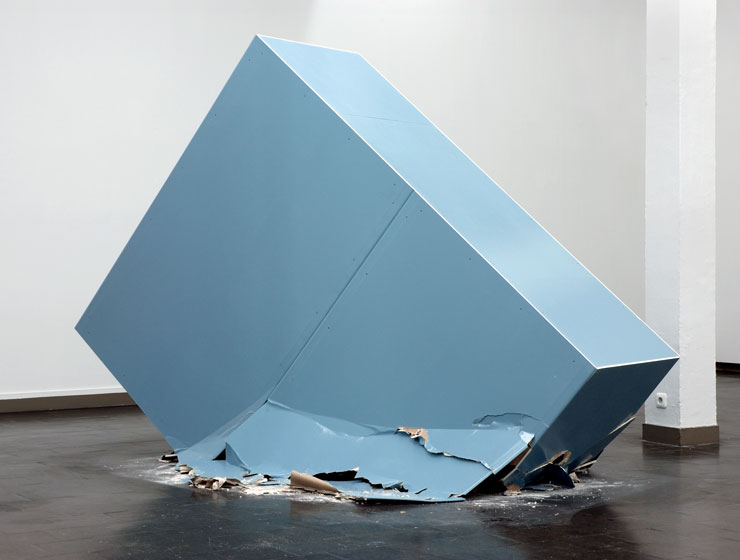
\includegraphics[scale=.7]{pictures/wickeroth-strategie-der-steine-3-2007}}

\end{frame}
\begin{frame}[t]\frametitle{Measurement Error}

Measurement error in classical content analysis is primarily failure of \textit{this} assumption:
\begin{center}
\begin{tabular}{lcc} \toprule
& $P(Z=\text{\textsl{state reg}}\mid \text W)$ & $P(Z=\text{\textsl{market econ}} \mid \text W)$ \\ \midrule
\text{age} & 1 & 0 \\
\text{benefit} & 1 & 0 \\
\ldots & \ldots & \ldots\\
\text{assets} & 0 & 1 \\
\text{bid} & 0 & 1\\
\ldots & \ldots & \ldots\\ \bottomrule
\end{tabular}
\end{center}

%\slide{Measurement Error}
%
%What are the effects of measurement error in category counts?
%
%\ita
%\itm Being directly wrong: My estimated rates are too \textit{low}
%\itm Being indirectly wrong: My constructed left-right measure is too \textit{centrist}
%\itz

\end{frame}
\begin{frame}[t]\frametitle{Measurement Error}

What are the effects of measurement error in category counts?

\ita
\itm Being directly wrong, e.g.
\ita
\itm My estimated rates are too \textit{low} (bias)
\itm Some of my estimates are more biased than others
\itz
\itm Being indirectly wrong, e.g.
\ita
\itm My carefully constructed left-right measure is too \textit{centrist}
\itm My effect sizes appear to be much too small
\itz
\itz


\end{frame}
\begin{frame}[t]\frametitle{Measurement Error}

Assume
\ita
\itm Vocabulary of only two words `benefit' and `assets'
\itm a \textit{subtractive} measure of position: $Z_{\text{\textsl{market econ}}} - Z_{\text{\textsl{state reg}}}$
\itz
Then
\begin{center}
\begin{tabular}{lcc} \toprule
& $P(Z=\text{\textsl{state reg}}\mid \text W)$ & $P(Z=\text{\textsl{market econ}} \mid \text W)$ \\ \midrule
\text{benefit} & 1 & 0 \\
\text{assets} & 0 & 1 \\
\bottomrule
\end{tabular}
\end{center}

\end{frame}
\begin{frame}[t]\frametitle{Measurement Error}

implies the \textbf{confusion matrix}

\begin{center}
\begin{tabular}{lrll} \toprule
& & True & \\\midrule
& & \textsl{state reg} & \textsl{market econ} \\ \midrule
Observed & \textsl{state reg}  & 1      & 0 \\
& \textsl{market econ}  & 0      & 1 \\ \bottomrule
\end{tabular}
\end{center}




\end{frame}
\begin{frame}[t]\frametitle{Measurement Error}

Example: What if $P(W \mid Z)$ slips to
\begin{center}
\begin{tabular}{rcc} \toprule
& \textsl{state reg} & \textsl{market econ} \\ \midrule
$P(\text{benefit} \mid \text{Z})$ & 0.7 & 0.2 \\
$P(\text{assets} \mid  \text{Z})$ & 0.3 & 0.8 \\ \bottomrule
\end{tabular}
\end{center}

~\\
P(W=`asset' | Z=\textsl{state reg}) > 0 so

P(Z=\textsl{state reg} | W=`asset') < 1

\end{frame}
\begin{frame}[t]\frametitle{Measurement Error}

When $Z_{\text{\textsl{market econ}}}=10$ and $Z_{\text{\textsl{state reg}}}=20$ the true difference is
\ita
\itm (10-20)/(10+20) = -0.33
\itz
Under the perfect measurement model this would be realised (on average) as
\ita
\itm 20 `benefit's and 10 `assets'
\itz

\end{frame}
\begin{frame}[t]\frametitle{Measurement Error}

Under our \textit{imperfect} measurement it is realised (on average) as
\ita
\itm 16 `benefit's (14 from \textsl{state reg} but 2 from \textsl{market econ}) and
\itm 14 `assets' (8 from \textsl{market econ} but 6 from \textsl{state reg})
\itz

\end{frame}
\begin{frame}[t]\frametitle{Measurement Error}

The proportional difference measure is now (14-16)/(14+16) = -0.07
\ita
\itm Apparently much closer to the centre, but only because of measurement error
\itz

\textit{All} relative measures will have this problem




\end{frame}
\begin{frame}[t]\frametitle{In Action (Laver and Garry 2000)}

\centerline{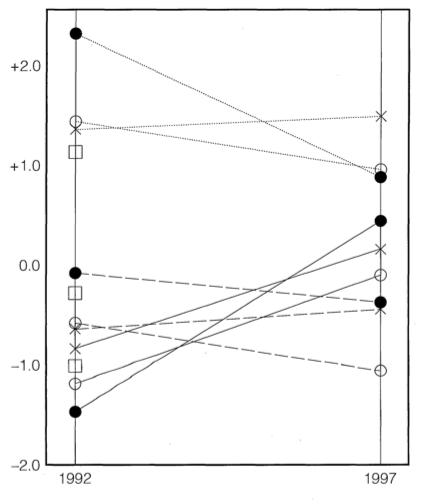
\includegraphics[scale=.7]{pictures/lg-shrinkage}}


\end{frame}
\begin{frame}[t]\frametitle{In Action (Mikhaylov et al. 2012)}

\centerline{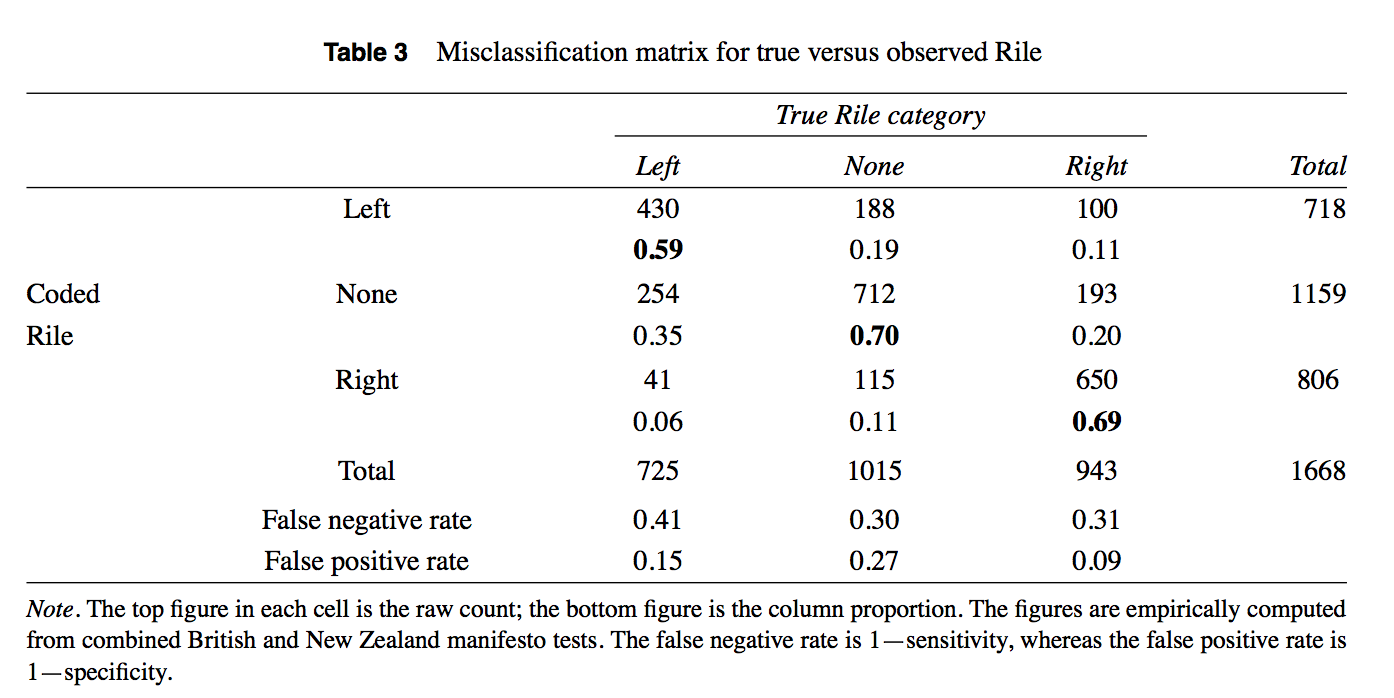
\includegraphics[scale=.9]{pictures/slava-rile3}}

\end{frame}
\begin{frame}[t]\frametitle{In Action (Mikhaylov et al. 2012)}

\centerline{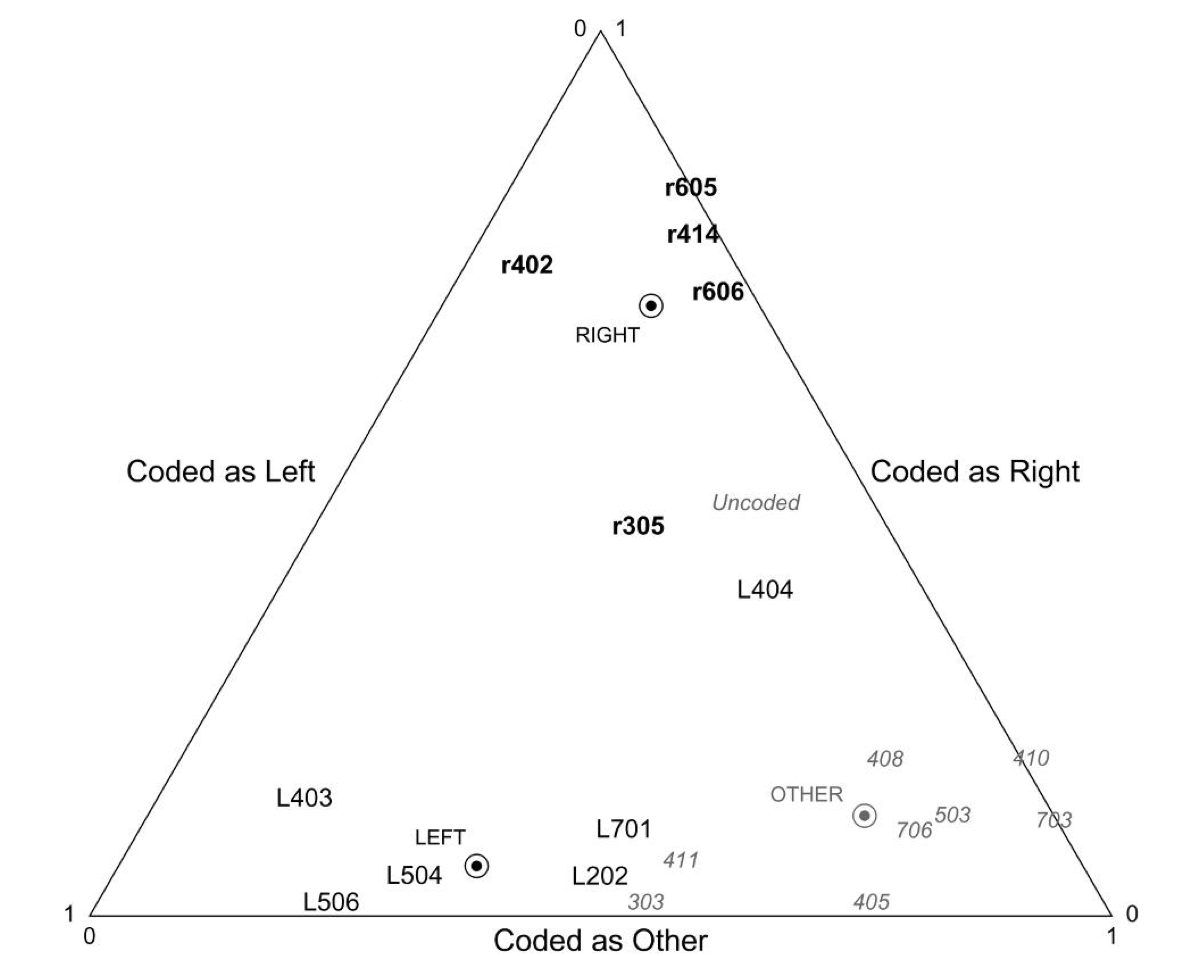
\includegraphics[scale=.7]{pictures/slava-rile2}}

\end{frame}
\begin{frame}[t]\frametitle{In Action (Mikhaylov et al. 2012)}

\centerline{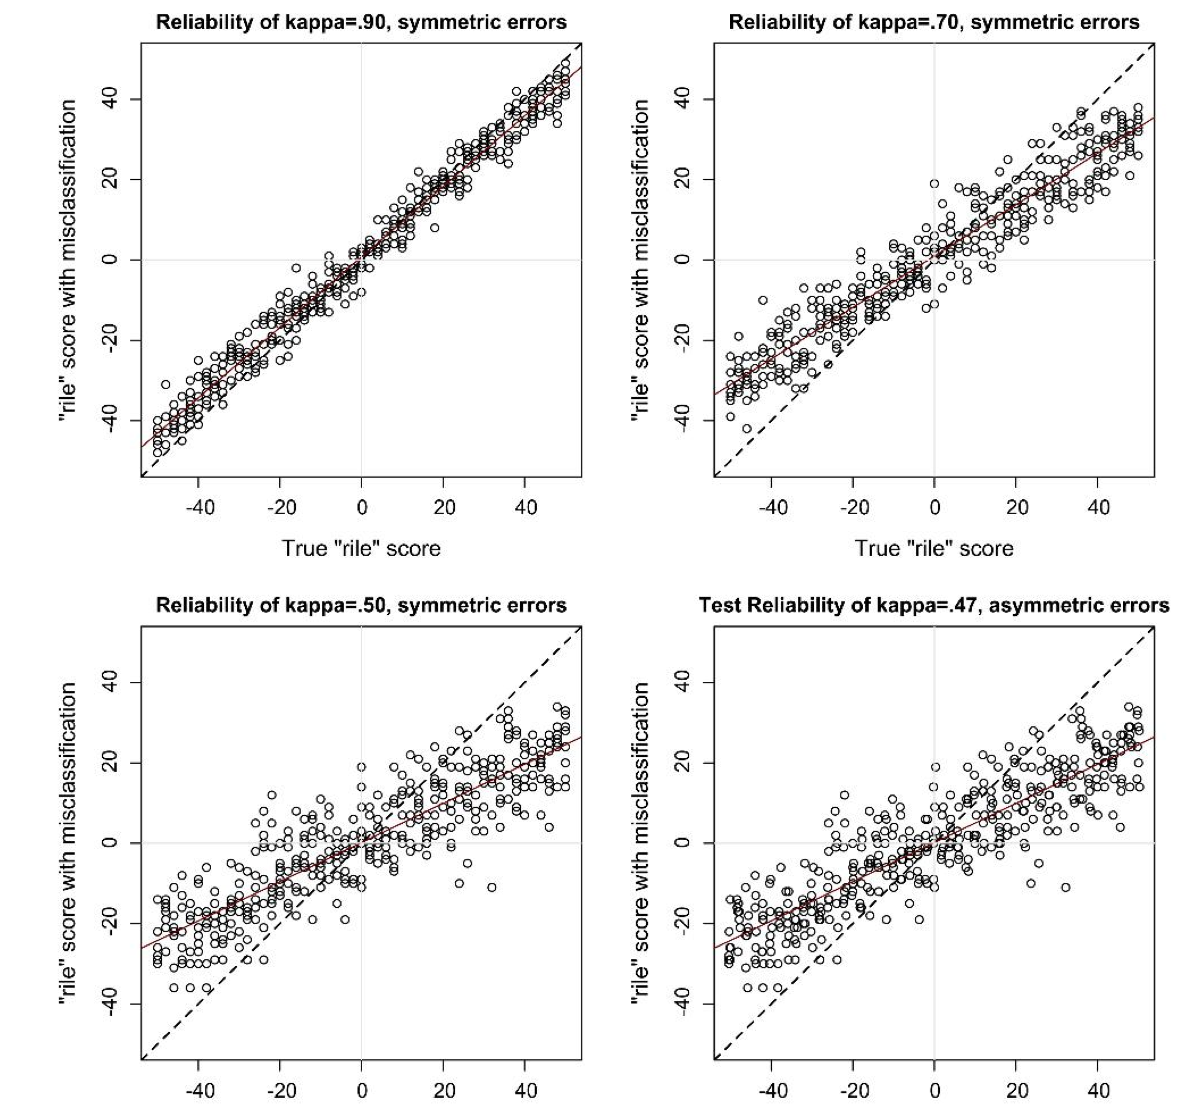
\includegraphics[scale=.6]{pictures/slava-rile}}


\newpage
\centerline{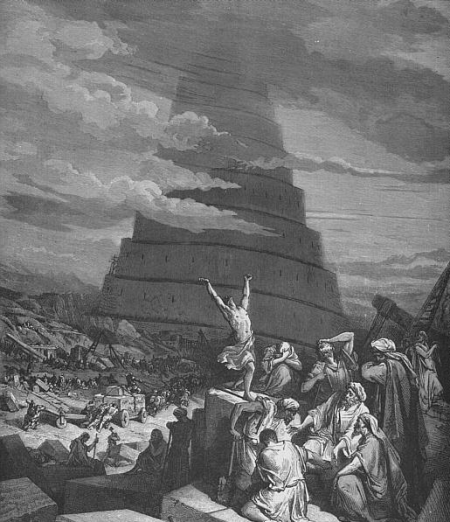
\includegraphics[scale=1]{pictures/confusionoftongues.png}}


\end{frame}
\begin{frame}[t]\frametitle{Solutions}

\newpage

\centerline{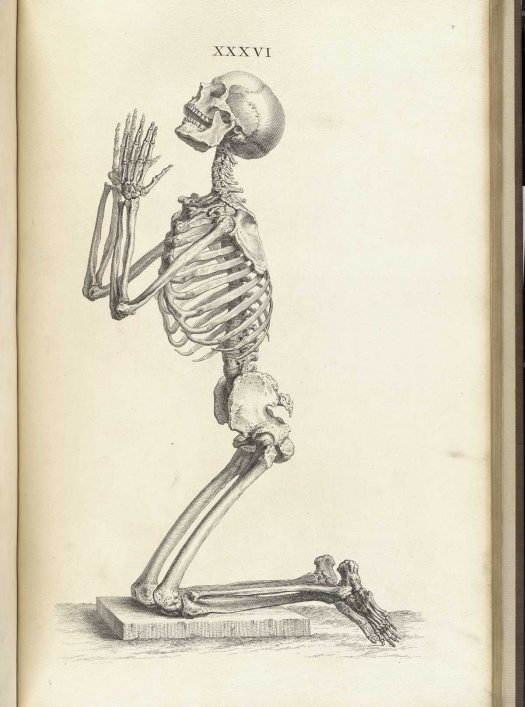
\includegraphics[scale=.7]{pictures/praying-skeleton}}

\end{frame}
\begin{frame}[t]\frametitle{Solutions: Try to Avoid it}

A non-intuitive fact about content dictionaries:
\ita
\itm \textbf{Precision}: proportion of words used the way your dictionary assumes
\itm \textbf{Recall}: proportion of words used that way that are in your dictionary
\itz
\textit{always} trade-off\ldots

\end{frame}
\begin{frame}[t]\frametitle{Intuition: Precision and Recall}

\centerline{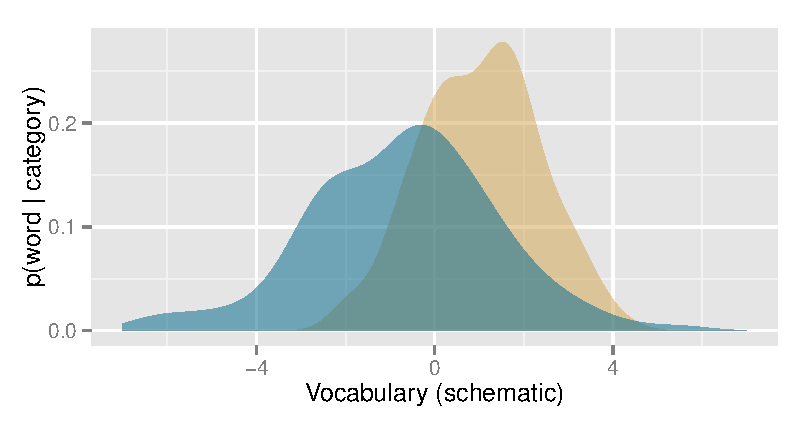
\includegraphics[scale=1.7]{pictures/schematic-vocab}}

\end{frame}
\begin{frame}[t]\frametitle{Solutions: Try to Avoid it}

Keyword in context analyses allow you to scan all contexts of a word
\ita
\itm How many of them are the sense or usage you want?
\itz

Compromise: KWIC analyses allow you to scan all contexts of a word
\ita
\itm What proportion of tokens are the sense or usage you want?
\itz

\newpage

\centerline{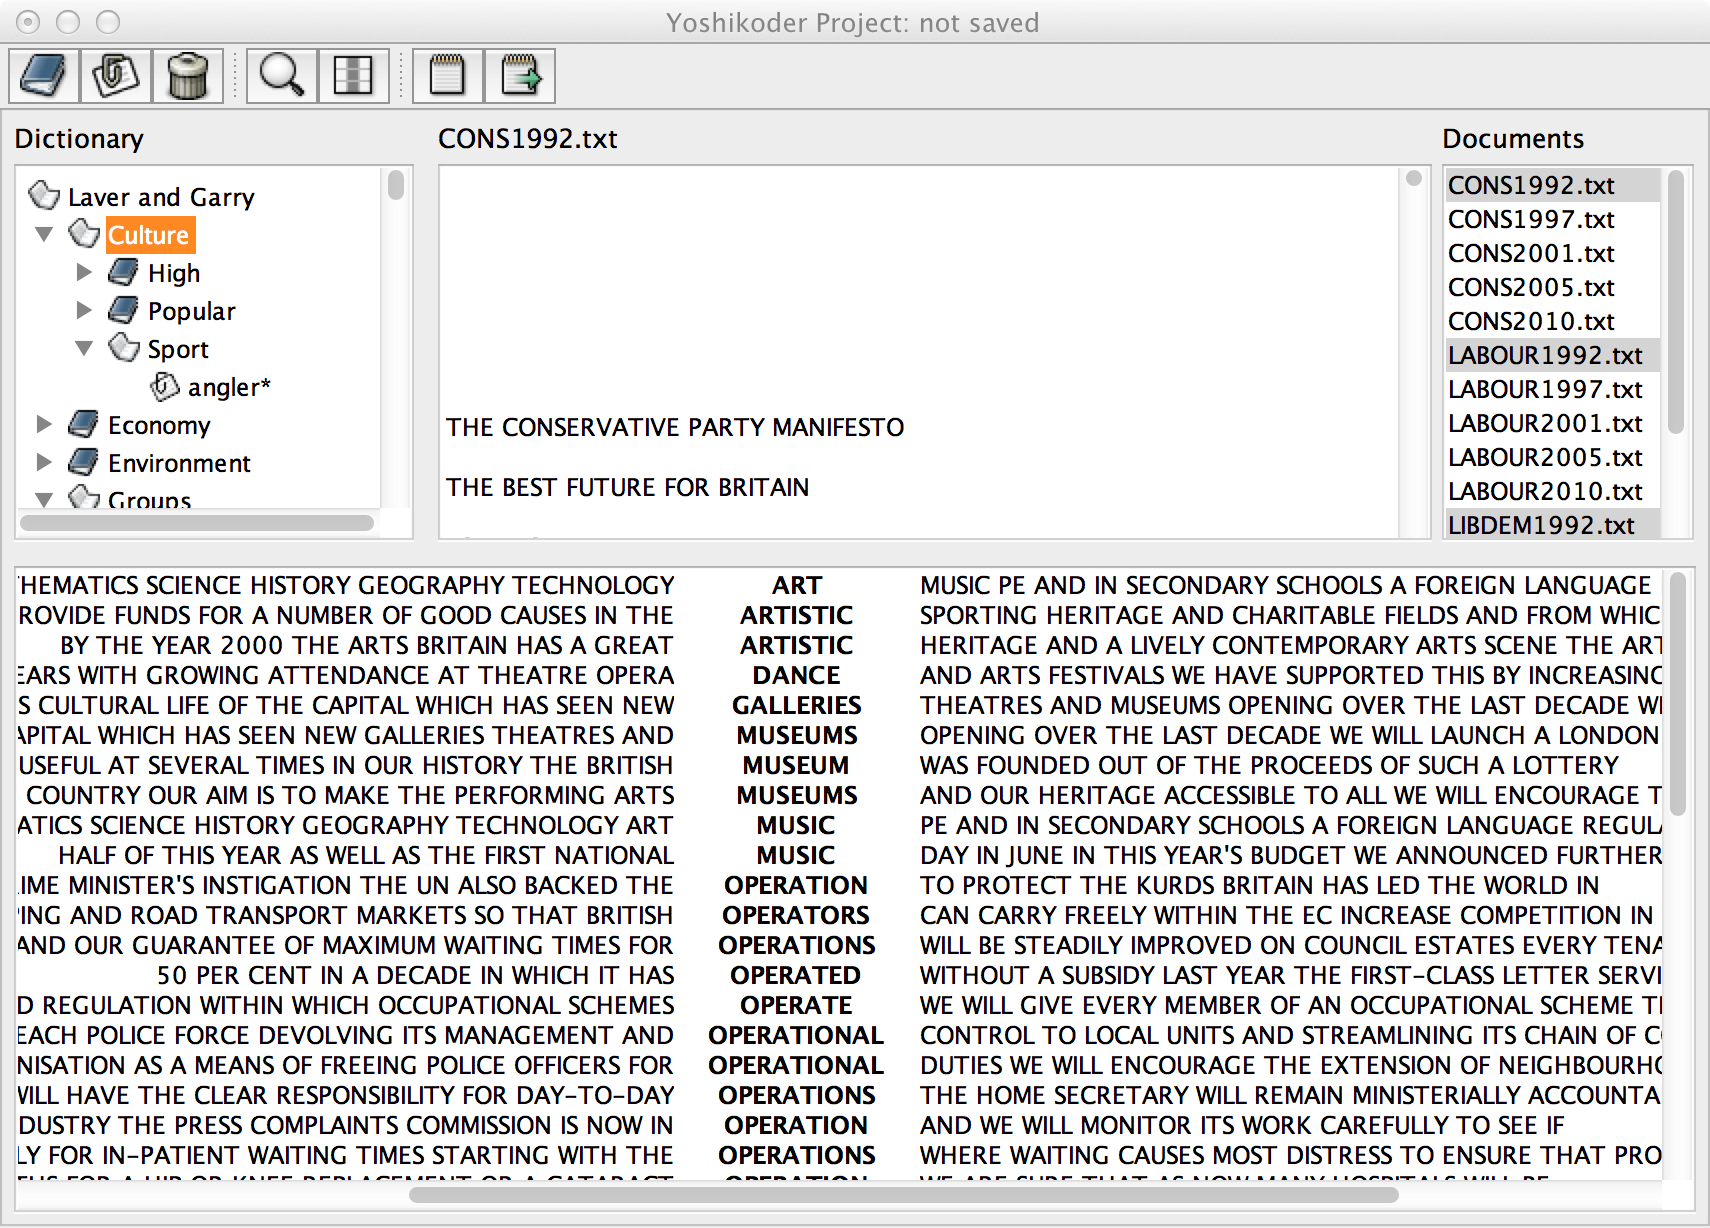
\includegraphics[scale=.7]{pictures/yk-measurement-error}}

\end{frame}
\begin{frame}[t]\frametitle{Recovering from Measurement Error: Model it (1)}

We can recover from measurement error if we know enough about it (Hopkins and King 2010, King and Liu 2007)

Coder training provides information about how a category proportion estimate changes as coders get better

Intuition:
\ita
\itm Model this trajectory, then extrapolate it forwards\ldots
\itz

In regression contexts this is called SIMEX (Cook and Stefanski, 1995).

\end{frame}
\begin{frame}[t]\frametitle{Recovering from Measurement Error: Model It (1)}

\centerline{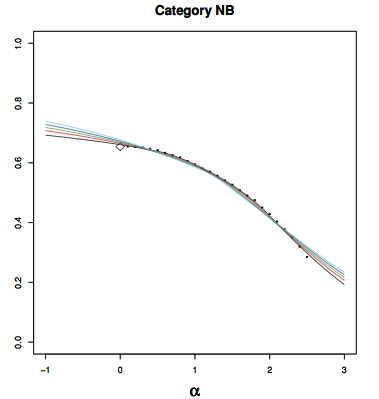
\includegraphics[scale=.8]{pictures/simex-proportion-hopkins-king}}

\end{frame}
\begin{frame}[t]\frametitle{Recovering from Measurement Error: Model It (2)}

Under measurement error
\ita
\itm A observed category proportions are generated by a \textit{mixture} of categories
\itm The weights for this mixture are the true category proportions
\itz
Given the confusion matrix (or the true generation probabilities), we can \textit{infer} the true proportions

\end{frame}
\begin{frame}[t]\frametitle{Recovering from Measurement Error: Model It (2)}

Intuition
\[
{P(W)} = \sum^K_k {P(W \mid Z=k)} P(Z=k)
\]
has the form
\[
Y = X\theta
\]
\[
\left[\begin{array}{c}0.53 \\0.46\end{array}\right] =
\left[\begin{array}{cc}0.7 & 0.2 \\0.3 & 0.8\end{array}\right] \left[\begin{array}{c}\theta_1 \\\theta_2\end{array}\right]
\]

is solved as [0.67, 0.33]

\end{frame}
\begin{frame}[t]\frametitle{Recovering from Measurement Error: Model It (2)}

Applied to Mikhaylov error data:

If $(P, T)$ is

\begin{tabular}{rrrr}
\hline
& L & N & R \\
\hline
L & 430.00 & 188.00 & 100.00 \\
N & 254.00 & 712.00 & 193.00 \\
R & 41.00 & 115.00 & 650.00 \\
\hline
\end{tabular}

\newpage

So $P(C \mid T)$ is

\begin{tabular}{rrrr}
\hline
& L & N & R \\
\hline
L & 0.59 & 0.19 & 0.11 \\
N & 0.35 & 0.70 & 0.20 \\
R & 0.06 & 0.11 & 0.69 \\
\hline
\end{tabular}

Implication:

If [L, N, R] = [20, 0, 10]
\ita
\itm we would expect to see about [13, 9, 8]
\itz

\newpage
Invert $P(C \mid T)$:

\begin{tabular}{rrrr}
\hline
& L & N & R \\
\hline
L & 2.00 & -0.50 & -0.16 \\
N & -1.00 & 1.75 & -0.37 \\
R & 0.00 & -0.25 & 1.52 \\
\hline
\end{tabular}

and multiply to get an estimate of the true counts\ldots

Example:
\ita
\itm Given counts [13, 9, 8] we get
\itm [L 20.19, -0.16,  9.98] $\approx$ [20, 0, 10]
\itz

\end{frame}
\begin{frame}[t]\frametitle{Notes:}

\ita
\itm This is all \textit{in expectation}.
\itm We are ignoring measurement error \textit{in the error matrix}
\itm This method may violate sensible prior information
\itm Works for anything that makes errors (human or machine)
\itz

\end{frame}
\begin{frame}[t]\frametitle{Recovering from Measurement Error: Model It (3)}

Topic models, e.g. Latent Dirichlet Allocation (Blei et al.) \textbf{add}:
\ita
\itm A \textit{probabilistic} view of the relationship between W, Z and $\theta$
\itm Full statistical framework for learning most aspects of the relationship
\itz

\end{frame}
\begin{frame}[t]\frametitle{Topic Models as Classical Content Analysis}

From

\centerline{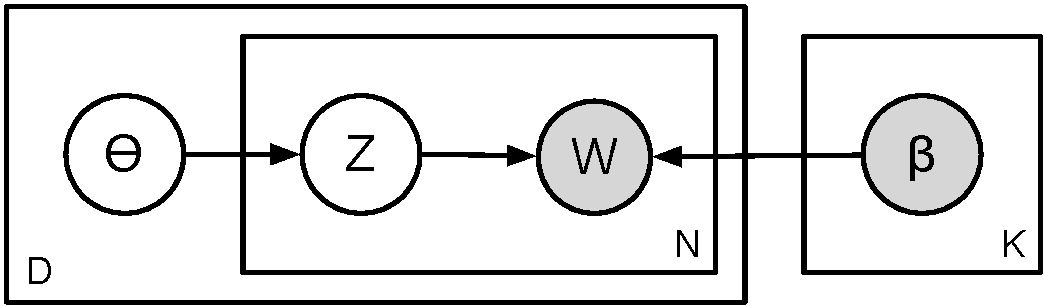
\includegraphics[scale=.8]{pictures/new-topics-ca}}

(via pLSI) to

\centerline{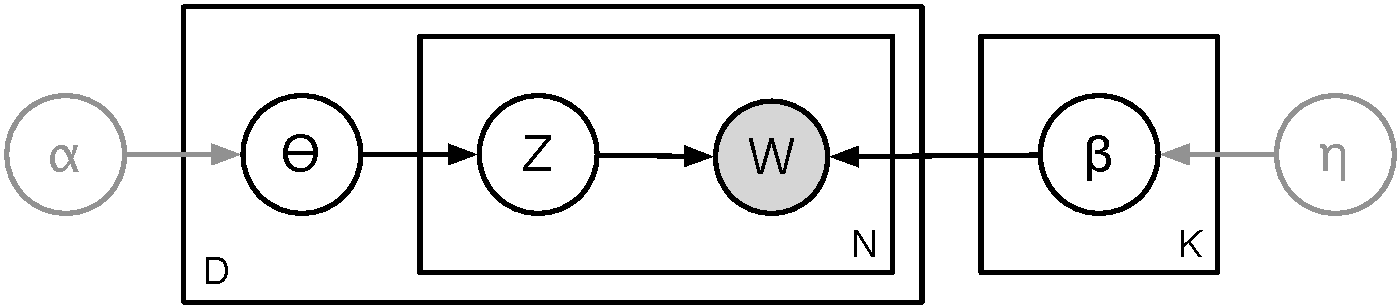
\includegraphics[scale=.8]{pictures/lda-flat}}

\end{frame}
\begin{frame}[t]\frametitle{Generative probability model}

Assumptions:
\ita
\itm W and Z are multinomial.
\itm $\theta$ and $\beta$ are Dirichlet
\itm $\alpha$ and $\eta$ are hyperparameters for Dirichlet parameters
\ita
\item Magnitude controls expected sparsity of words per topic and topics realised per document
\item Often optimised directly (a la `Empirical Bayes') rather than integrated out
\itz
\itz
%% Todo dirichlet parameters

\end{frame}
\begin{frame}[t]\frametitle{$\alpha=10$}

\centerline{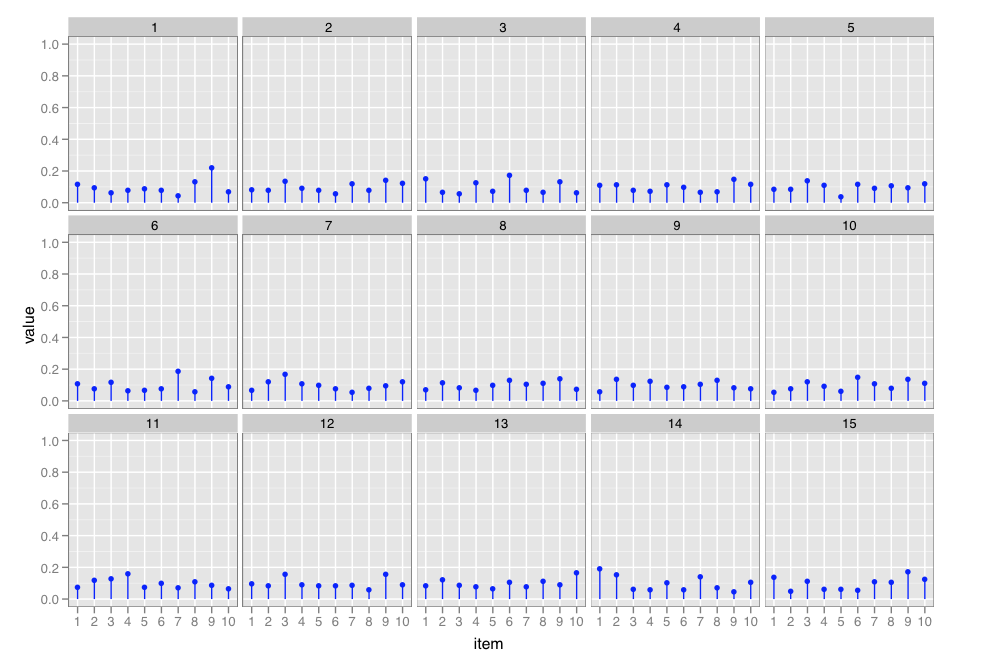
\includegraphics[scale=1]{pictures/dirichlet-alpha10}}

\end{frame}
\begin{frame}[t]\frametitle{$\alpha=.1$}

\centerline{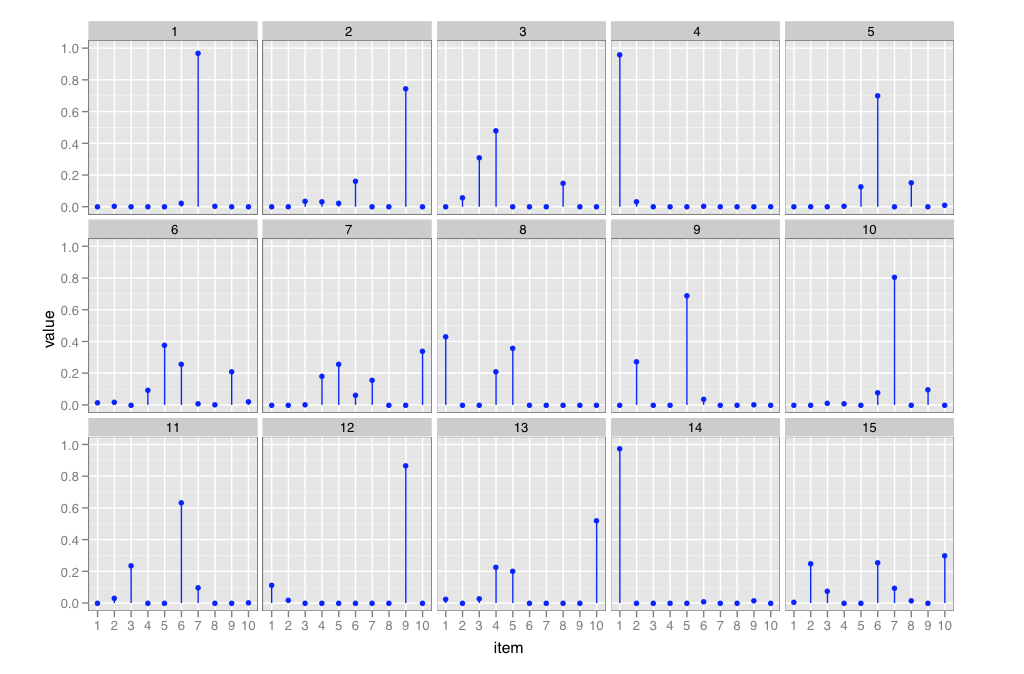
\includegraphics[scale=1]{pictures/dirichlet-alpha-tenth}}

%% todo correlated topic model next

%% todo the hyperspace planar picture

%% todo: measures of validity

%% -----------------

%\slide{Topic Models}
%\centerline{\includegraphics[scale=.6]{pictures/topic-model}}
%
%\slide{Recovering from Measurement Error: Model It (3)}
%
%Topic models, e.g. Latent Dirichlet Allocation (Blei et al.) \textbf{take away}:
%\ita
%\itm Substantive control: You do not get to assert what the topics \textit{mean}
%\itm This is inevitable when the Z and $\theta$ are both unobserved\ldots
%\itz
%
%
%Topic models (Blei, Ng and Jordan, 2003; Blei and Lafferty, 2009) are full probability models that
%\ita
%\itm weaken the constraints required in dictionary based content analysis
%\itm may do what you want.  Or not\ldots
%\itz
%
%These are \textit{exploratory} methods that work best
%with \textit{large amounts} of text with a \textit{thematic} structure.
%

%\slide{Topic Models: LDA}
%
%Topic models represent documents as a mixture of topics.
%
%All documents in the text collection (e.g. Congressional bills) share the same set of topics, but each document (e.g. individual bill) exhibits a different proportion of topics.
%
%
%
%Documents are observed, the rest is not:
%\ita
%\itm topics
%\itm the per-document topic distribution
%\itm  the per-document per-word topic assignment.
%\itz
%%\centerline{\includegraphics[scale=.6]{pictures/topic-model2}}
%
%\slide{Topic Models: LDA}
%
%
%\centerline{\includegraphics[scale=.6]{pictures/topics}}
%
%
%\slide{Topic Models: LDA}
%
%\centerline{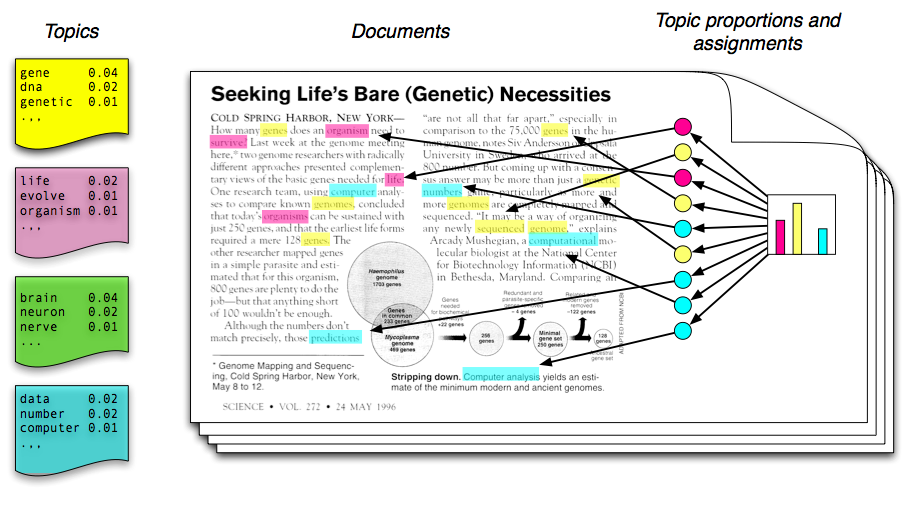
\includegraphics[scale=.6]{pictures/topics2}}
%
%
%\slide{Topic Models: LDA}
%
%Latent Dirichlet Allocation (LDA):
%
%Dirichlet distribution describes knowledge about a vector of probabilities, here the probabilities of topics per document.
%
%A generative model:
%
%For example, with two topics, you may choose that a document is 1/3 about topic A and 2/3 about topic B.
%
%\slide{Topic Models: LDA}
%
%\centerline{\includegraphics[scale=.6]{pictures/topic-model}}
%
%
%\slide{Topic Models: LDA}
%
%LDA reverses the generative process to find the hidden structure that is likely to have generated the observed documents (essentially using the co-occurrence of words across documents)
%
%
%Topic models add:
%\ita
%\itm A \textit{probabilistic} view of the relationship between W (observed word), Z (per-word topic assignment) and $\theta$ (per-document topic proportions)
%\itm Topics = distribution over a fixed vocabulary
%\itm Full statistical framework for learning most aspects of the relationship
%\itz
%
%\slide{Topic Models: LDA}
%
%But:
%\ita
%\itm topic models take away substantive control: you do not get to assert what the topics \textit{mean}
%\itm they return only one single clustering
%\itz

%\slide{Applications: Policy Agenda}


\end{frame}
\begin{frame}[t]\frametitle{Interpretation}

Topic assignment measurement process is modeled  (yay!)

Topic meaning is no longer under your control (boo!)

Topic modeling is (mostly) \textit{exploratory} rather than \textit{confirmatory}

Upshot:
\ita
\itm \textit{You} have to make the case that your topic model is capturing the topic you want to be capturing and not others.
\itm Topic \textit{number} is now an open question
\itz

\end{frame}
\begin{frame}[t]\frametitle{What is this topic anyway?}

\centerline{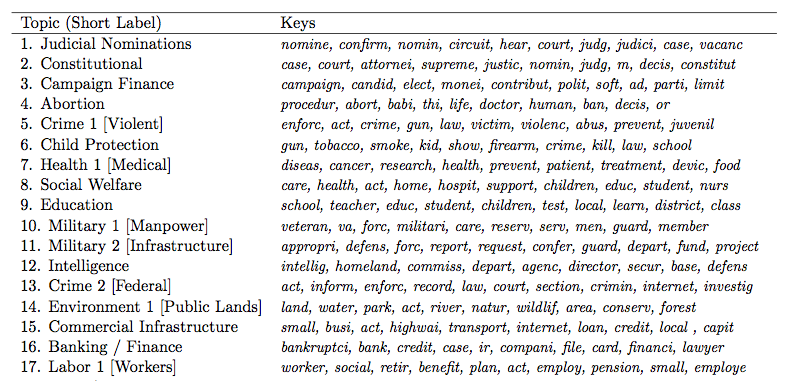
\includegraphics[scale=.8]{pictures/topic-words}}

{\footnotesize (Quinn et al. 2010)}

\end{frame}
\begin{frame}[t]\frametitle{How is it related to others topics?}

\centerline{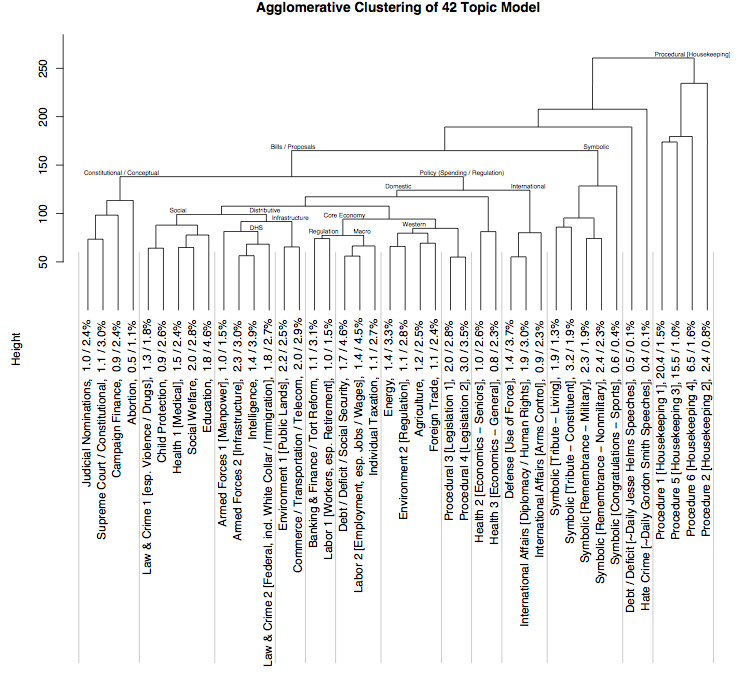
\includegraphics[scale=.55]{pictures/topic-clustering}}

\end{frame}
\begin{frame}[t]\frametitle{and other schemes?}

\centerline{\includegraphics[scale=.5]{pictures/other-schemes}}

%
%\slide{Variations: Expressed Agenda Model}
%
%In a simpler variation on LDA, Grimmer (2010) defines an expressed agenda model for Senate press releases. \vspace{5mm}
%~\\
%\centerline{\includegraphics[scale=2.2]{pictures/grimmer}}
%
% Here there are \textit{not} multiple topics per senatorial press release, but senators are at the mixed membership level (i.e. mix attention to topics).
%
%Goal: estimate the topics in the data (all Senate press releases), assign press releases to their likely topic, and measure attention  Senators dedicate to estimated topics.
%

\end{frame}
\begin{frame}[t]\frametitle{Topic Models: How \textit{many} topics?}

{\small
\begin{quote}
The results presented in this paper [\ldots] assume there are 43 topics present in the data. I varied the number of assumed topics from only five topics, up to 85 different topics. Assuming too few topics resulted in distinct issues being lumped together, whereas too many topics results in several clusters referring to the same issues. \textsl{During my tests, 43 issues represented a decent middle ground.}
(Grimmer 2010, p.12)
\end{quote}
}

\end{frame}
\begin{frame}[t]\frametitle{Nested topics?}

\centerline{\includegraphics[scale=.8]{pictures/nested-topics-nuclear}}

from Jacobi et al (2014) -- Hierarchical Dirichlet Process models models \textit{do} enforce nested topics

\end{frame}
\begin{frame}[t]\frametitle{A troubling tension}

There are two natural metrics for evaluating topic models (or any other kind of computer assisted text analysis)
\ita
\itm Statistical performance, e.g. held-out likelihood
\itm Substantive usefulness, e.g. topic coherence
\itz
Experiments by Chang et al. (2009), using
\ita
\itm word intrusion (which word does not belong?)
\itm topic intrusion (which topic does not belong?)
\itz
suggest that these are robustly \textit{negatively} correlated.



%\slide{Labeling topics}
%
%\begin{enumerate}
%\item Randomly select documents from each topic with a high posterior probability of belonging to that topic, then read and manually assign a label (compare cluster quality)
%\item Use the model output to identify words that distinguish the documents in a particular topic
%\item Validate with external events (predictive validity)
%\end{enumerate}

%\slide{Labeling Topics}
%
%\centerline{\includegraphics[scale=1.2]{pictures/grimmertopics}}
%
%\slide{Labeling Topics}
%
%
%\centerline{\includegraphics[scale=2]{pictures/grimmerimmig}}
%
%
%Senators issue press releases on the topic with the label "immigration" when important votes in the Senate take place.
%
%\slide{Assessing Validity of Topics}
%
%
%
%Expectation: Members of Congress want to be perceived as being effective policy makers and emphasize issues that come before committees they lead (Fenno 1978).
%
%Grimmer compares committee leaders' average attention to an issue under the committee's jurisdiction with the average attention among the other Senators.
%
%\slide{Assessing Validity of Topics }
%
%\centerline{\includegraphics[scale=0.9]{pictures/grimmercomm}}
%
%Committee leaders pay more attention to their committee's issues.
%
%\slide{Assessing Validity of Topics (Grimmer)}
%
%Expectation:  Senators who tout  appropriations secured for a state in their press releases view these appropriations essential to their electoral security and should be less likely to vote for earmark reform.\vspace{10mm}
%
%\centerline{\includegraphics[scale=1.5]{pictures/grimmerearmark}}


%%%%%%%%%%%%%%



\end{frame}
\begin{frame}[t]\frametitle{Variations}

There have been a huge number of variations on and extensions of the basic topic model
\ita
\itm Airoldi et al. 2011 Table 1 provide references for 33!
\itz
I'll briefly mention two variations of interest to political science:
\ita
\itm Dynamic topic models
\itm Structural topic models (\url{http://structuraltopicmodel.com})
\itz

\end{frame}
\begin{frame}[t]\frametitle{Dynamic Topic Models (1)}

Words `drift' from topic to topic over time

\centerline{\includegraphics[scale=.8]{pictures/blei-dynamic}}

\end{frame}
\begin{frame}[t]\frametitle{Dynamic Topic Models (1)}

\centerline{\includegraphics[scale=.7]{pictures/dynamics}}

\end{frame}
\begin{frame}[t]\frametitle{Dynamic Topic Models (2)}

Alternatively (Quinn et al 2010) document topic proportions `drift' over time
\ita
\itm To track a smoothly moving policy agenda (congressional speeches from 1997-2004)
\itz

\centerline{\includegraphics[scale=.5]{pictures/defence-topic-quinn}}

~\\
Note:
\ita
\itm It's not clear you can have both types of dynamics!
\itz

\end{frame}
\begin{frame}[t]\frametitle{Structural Topic Models}

\centerline{\includegraphics[scale=.6]{pictures/stm-graphical-model}}

Covariates for topics proportions and on topic words

\end{frame}
\begin{frame}[t]\frametitle{Structural Topic Models}

Think SEM/Multilevel measurement models for text\ldots

Some history of modeling topic proportions:
\ita
\itm LDA: Topic proportions are \textit{nearly} a priori independent
\itm CTM `Correlated Topic Model': Topic proportions can be correlated via a Normal distribution in the space of topic proportion logits
\itm STM `Structural Topic Model': Topic proportion correlations are regressions on covariates
\itz

Covariates are intended to facilitate interpretation/explanation (also provide measurement bias)

\end{frame}
\begin{frame}[t]\frametitle{Structural Topic Models}

\centerline{\includegraphics[scale=.8]{pictures/stm-clerics}}

\end{frame}
\begin{frame}[t]\frametitle{Wrapping up}

\centerline{\includegraphics[scale=1.5]{pictures/compromise.png}}


\end{frame}
\begin{frame}[t]\frametitle{Lab Time}

\centerline{\includegraphics[scale=.8]{pictures/hieroglyphic-keyboard-cm}}


%
%\slide{Recovering from Measurement Error: Model It}
%
%Intuition
%\[
%{P(W)} = \sum^K_k {P(W \mid Z=k)} P(Z=k)
%\]
%has the form
%\[
%Y = X\theta
%\]
%In our example:
%
%\[
%\left[\begin{array}{c}0.53 \\0.46\end{array}\right] =
%\left[\begin{array}{cc}0.7 & 0.2 \\0.3 & 0.8\end{array}\right] \left[\begin{array}{c}\theta_1 \\\theta_2\end{array}\right]
%\]
%
%is solved is as [0.67, 0.33]
%
%\slide{Recovering from Measurement Error: Correct It}
%
%We can recover from measurement error if we know enough about it (Hopkins and King 2010, King and Liu 2007)
%
%Under measurement error
%\ita
%\itm A observed category proportions are generated by a \textit{mixture} of categories
%\itm The weights for this mixture are the true category proportions
%\itz
%Given the confusion matrix (or the true generation probabilities), we can \textit{back out} the true proportions
%





%%%%%%%%%%

%
%
%\slide{Doing it Yourself}
%
%Building and applying content analysis dictionaries: Yoshikoder (Hamlet, Wordstat, MaxQDA)
%
%Turning things into text: YKConverter, pdftotext
%
%~\\
%All available (for free) at http://conjugateprior.org
%
%
%
%
\end{frame}
\end{document}

%
%%%%%%%%%%%%%%%%%%%%%%%%%
%%%%%%%%%%%%%%%%%%%%%%%%%
%%%%%%%%%%%%%%%%%%%%%%%%%
%
%
%
%\slide{Regression Approaches}
%
%If we can't provide a dictionary, we can try to \textit{infer} a dictionary
%
%Text classification:
%\ita
%\itm Assume $Z$ is a category label (nominal dependent variable)
%\itm Assume we have some texts that with \textit{known} $Z$s
%\itm We can sometimes learn the classification function, e.g.
%\begin{equation*}
%P(Z \mid W_i \ldots W_V) ~=~ \text{logit}^{-1}(\alpha + \beta_1 W_1 + \beta_2 W_2 + \ldots)
%\end{equation*}
%\itz
%
%\slide{Regression Approaches}
%
%Example: Amicus Curiae briefs for 3 supreme Court affirmative action cases from (Evans et al.)
%\ita
%\itm Which words make a brief 'liberal' or 'conservative'?
%\itm Use the parties own briefs to estimate the model
%\itm Classify the briefs
%\itz
%
%\slide{Regression Approaches}
%
%\begin{center}
%\includegraphics[scale=.6]{pictures/words-evans}
%\end{center}
%
%\slide{Compare and Contrast}
%
%Bara et al. (2007) analyse 1966 abortion debate in the House of Commons with a thematic CA dictionary
%\begin{center}
%\includegraphics[scale=.6]{pictures/bara-diffs}
%\end{center}
%
%
%\slide{Regression Approaches}
%
%But what if we \textit{don't have} any texts with known $Z$?
%
%Try to \textit{learn} a `dictionary'\ldots
%
%\slide{Topic models}
%
%A type of latent class model
%\ita
%\itm $\theta$ is a set of topic proportions (with labels Z)
%\itm Assume we know the number of topics, \textit{but not their content}
%\itm For each topic, words are Multinomially distributed i.e. they have their own set of word probabilities $\pi_1 \ldots \pi_V$
%\itm A document is an unknown mix of topics
%\itz
%
%In topic models, word occurrences depend on which topic generated them = which topic they are being used to express
%
%\slide{Topic models}
%
%\begin{center}
%\includegraphics[scale=.6]{pictures/topics2}
%\end{center}
%
%\slide{Topic models}
%
%\begin{center}
%\includegraphics[scale=.6]{pictures/topic-model}
%\end{center}
%
%\slide{Legislative Debate}
%
%\begin{center}
%\includegraphics[scale=.5]{pictures/911}
%\end{center}
%
%\slide{Legislative Vocabulary}
%
%\begin{center}
%\includegraphics[scale=.8]{pictures/topic-words}
%\end{center}
%
%\slide{}
%
%
%
%\slide{Tomorrow}
%
%~\\
%What if $\theta$ is not a topic proportion, but rather a \textit{position}
%
%That's all for tomorrow\ldots
%
%
%
%\end{document}
%
%%%%%%%%%%%%%%%%%%%%%%%%
%%% part 2 %%%%%%%%%%%%%
%%%%%%%%%%%%%%%%%%%%%%%%
%
%
%
%%%%%%% Measurement here
%
%
%\slide{Measurement models}
%
%Substantive assumption
%\begin{quotation}
%\noindent
%Unobserved $\theta$ \textsl{causes} observations $W_1, W_2, W_3,\ldots, W_V$
%\end{quotation}
% Statistical assumption
%\begin{quotation}
%$P(W_1,\ldots, W_V \mid \theta) ~=~ \prod_w^{V} P(W_w \mid {\theta})$
%\end{quotation}
%Once $\theta$ is known, variation in $W_1, W_2, W_3,\ldots, W_V$
%is random.
%
%\slide{Measurement models}
%
%General Principle:
%\ita
%\itm Effects of a common cause will be correlated, until it is conditioned on, or controlled for
%\itz
%
%You've seen this before, e.g
%\ita
%\itm good regression models make observations random, conditional on the explanatory variables
%\itz
%
%
%\slide{Measurement Models}
%
%Measurement model:
%\ita
%\itm Fit a model of $W_1 \ldots W_V \Leftarrow \theta$\\
%then \textit{reverse} it to get an estimate of $\theta$
%\itz
%Examples:
%\ita
%\itm Factor Analysis
%\itm Latent Class analysis
%\itm Item Response Theory
%\itm Structural Equation Models
%\itz
%
%\slide{Measurement Models}
%
%Advantage: Requires no information about $Z$s or $\theta$s
%
%Disadvantage: Leans heavily on functional and distributional assumptions
%
%Let's look at some possible assumptions\ldots
%
%\slide{How might $\theta$ affect words?}
%
%word prob. depends on \textit{identity} of $\theta$\\
% (via a category label Z)
%
%word prob. depends on the \textsl{magnitude} of $\theta$
%
%word prob. depends on the \textsl{distance} of $\theta$ from a point
%
%
%
%%%%%%%%%%%%%%% scaling %%%%%%%%%%%%%
%
%\slide{Of Left and Right}
%
%
%Spatial politics assumptions:
%\ita
%\itm Policy preferences are \textit{positions} or \textit{ideal points} on policy \textit{dimensions}
%\itm There exists a \textit{low-dimensional space} that explains the multitude of positioning information available in observations of politics
%\itz
%Take everyday talk about 'left' and 'right' seriously.
%
%Political representation is effective -- democratic, legitimate -- if politicians' preferences have the \textsl{right relationship} to citizens' preferences.
%
%\slide{Raw Materials of Left and Right}
%
%Quantitative positioning information:
%\ita
%\itm Votes in a legislature (obvious, but biased)
%\itm Answers to survey questions (unbiased but only sometimes possible)
%\itm Structured qualitative analysis of manifestos (e.g. Pellican, Krouwel)
%\itm Counts of policy promises or assertions in a manifesto or speech (Budget et al.)
%
%\itm Frequencies of individual words
%\itz
%
%\slide{Of Left and Right}
%
%\begin{center}
%\includegraphics[scale=.3]{pictures/local-maastricht}
%\end{center}
%
%
%Keiskompass (see also Wahl-o-mat).
%
%
%\slide{Senate Speeches (Monroe et al.)}
%
%\begin{center}
%\includegraphics[scale=.2]{pictures/senator-ip-monroe-maeda}
%\end{center}
%
%\slide{UK and IE Parties on the Economy}
%
%\begin{center}
%\includegraphics[scale=.25]{pictures/wordscores-uk-ie}
%\end{center}
%
%
%\slide{2009 IE Budget Debate}
%
%\begin{center}
%\includegraphics[scale=.6]{pictures/clean-snap}
%\end{center}
%
%\slide{Scaling Model (Proksch and Slapin)}
%
%Assumptions about $P(W_1\ldots W_V \mid \theta)$
%\begin{align*}
%\log  \lambda_{ij} &~=~ \psi_j ~+~ \beta_j\theta_i ~+~  \alpha_i
%\end{align*}
%
%$\theta_i$ is the expressed position of a text
%
%\slide{Scaling Model (Proksch and Slapin)}
%
%Assumptions about $P(W_1\ldots W_V \mid \theta)$
%\begin{align*}
%\log  \lambda_{ij}  &~=~ \psi_j ~+~ \beta_j\theta_i ~+~  \alpha_i
%\end{align*}
%
%$\alpha_i$ is a constant term controlling for document length
%
%\slide{Scaling Model (Proksch and Slapin)}
%
%Assumptions about $P(W_1\ldots W_V \mid \theta)$
%\begin{align*}
%\log  \lambda_{ij}  &~=~ \psi_j ~+~ \beta_j\theta_i ~+~  \alpha_i
%\end{align*}
%
% The \textsl{sign} of $\beta_j$ represents the \textsl{ideological direction} of $W_j$
%
%\slide{Scaling Model (Proksch and Slapin)}
%
%Assumptions about $P(W_1\ldots W_V \mid \theta)$
%\begin{align*}
%\log  \lambda_{ij}  &~=~ \psi_j ~+~ \beta_j\theta_i ~+~  \alpha_i
%\end{align*}
%
% The \textsl{magnitude} of $\beta_j$ represents the \textsl{sensitivity} of the word to ideological differences among speakers or parties
%
%\slide{Scaling Model (Proksch and Slapin)}
%
%Assumptions about $P(W_1\ldots W_V \mid \theta)$
%\begin{align*}
%\log  \lambda_{ij}  &~=~ \psi_j ~+~ \beta_j\theta_i ~+~  \alpha_i
%\end{align*}
%
%$\psi_j$ is a constant term for the word (larger for high frequency words).
%
%
%\slide{Scaling Model (Proksch and Slapin)}
%\begin{center}
%\includegraphics[scale=.3]{pictures/log-lambda.pdf}\hfill
%\includegraphics[scale=.3]{pictures/lambda.pdf}
%\end{center}
%
%The underlying Poisson regression model reflects a \textit{multiplicative} relationship between position and words used
%
%\slide{Marginal Effects}
%
%British National Party manifesto for 2009 EU elections
%
%\slide{Marginal Effects}
%
%\footnotesize
%Immigration is out of control.
%\normalsize
%
%\slide{Marginal Effects}
%
%\footnotesize
%Immigration is out of control.
%\textbf{Britain's population is now over 60 million and rising, solely due to immigration.}
%\normalsize
%
%\slide{Marginal Effects}
%
%\footnotesize
%Immigration is out of control.
%Britain's population is now over 60 million and rising, solely due to immigration.
%\textbf{Not only is Britain increasingly overcrowded but the fact is that a country is the product of its people  and
%if you change the people you will inevitably change the nature of the country.}
%\normalsize
%
%\slide{Marginal Effects}
%
%\footnotesize
%Immigration is out of control.
%Britain's population is now over 60 million and rising, solely due to immigration.
%Not only is Britain increasingly overcrowded but the fact is that a country is the product of its people  and
%if you change the people you will inevitably change the nature of the country.
%\textbf{We want Britain to remain - or return to - the way it has traditionally been.}
%\normalsize
%
%\slide{Marginal Effects}
%
%\footnotesize
%Immigration is out of control.
%Britain's population is now over 60 million and rising, solely due to immigration.
%Not only is Britain increasingly overcrowded but the fact is that a country is the product of its people  and
%if you change the people you will inevitably change the nature of the country.
%We want Britain to remain - or return to - the way it has traditionally been.
%\textbf{We accept that Britain will always have ethnic minorities and
%have no problem with this as long as they remain minorities and
%neither change nor seek to change the fundamental culture and identity of the indigenous peoples of the British Isles.}
%\normalsize
%
%\slide{Marginal Effects}
%
%\footnotesize
%\ldots fundamental culture and identity of the indigenous peoples of the British Isles.
%\textbf{The current open-door policy and unrestricted uncontrolled immigration is leading to higher crime rates, demand for more housing (driving prices out of the reach of young people), severe strain on the environment, traffic congestion, longer hospital waiting list, lower educational standards, higher income taxes, lower wages, higher unemployment, loss of British identity, a breakdown in community spirit, more restrictive policing, higher council tax rates, a shortage of council homes, higher levels of stress and unhappiness and a more atomized society.}
%\normalsize
%
%\slide{Marginal Effects}
%
%~\\
%Are we getting the point yet?
%
%%\itm {sentence counts} (Budge 1994; Elff 2008)
%
%\slide{}
%
%\begin{center}
%\includegraphics[scale=.35]{pictures/sp-informativeness.png}
%\end{center}
%
%\slide{Whew!}
%
%~\\
%For the slower version, attend the ECPR Ljubljana Summer School in Methods and Techniques
%
%Questions? Feuer frei!
%
%
%
%
%\end{document}
